\documentclass[lineno]{jfm}
\usepackage{graphicx}
\usepackage{multirow}
\usepackage{caption}
\usepackage{subcaption}
\usepackage{booktabs}
\usepackage{float}
\usepackage{cancel}
\usepackage[normalem]{ulem}   % normalem: keeps \emph{} italic instead of underlined
\usepackage{newtxtext}
\usepackage{newtxmath}
\usepackage{natbib}
\usepackage{comment}
\usepackage{hyperref}
\hypersetup{
    colorlinks = true,
    urlcolor   = blue,
    citecolor  = black,
}
\newtheorem{lemma}{Lemma}
\newtheorem{corollary}{Corollary}
\newtheorem{remark}{Remark}

% ---- Editorial macros -------------------------------------------------------
% \orn / \cbp are kept for the authors' workflow. In this revision they are used
% ONLY for genuinely open questions that require an author decision; text that
% was previously wrapped in them and is now settled has been promoted to plain
% black body text.
\newcommand{\orn}[1]{{\color{red} \textbf{[Oscar:} #1\textbf{]}}}
\newcommand{\cbp}[1]{{\color{blue} \textbf{[Carlos:} #1\textbf{]}}}
\newcommand{\coor}[1]{{\color{blue} #1}}
\newcommand{\todo}[1]{{\color{red} \textbf{[TODO:} #1\textbf{]}}}
\newenvironment{cbpblock}%
  {\par\color{blue}\noindent\textbf{[Carlos]}\ \ignorespaces}%
  {\par}
\newenvironment{ornblock}%
  {\par\color{red}\noindent\textbf{[Oscar]}\ \ignorespaces}%
  {\par}
% -----------------------------------------------------------------------------

\title{An analytical constitutive-to-resistance closure for Windkessel
haemodynamics with generalised-Newtonian rheology}

\author{Carlos Brito-Pacheco\aff{1}, Milenko Espinosa\aff{2},
  Ernesto Castillo\aff{2}, Scarlett Espinoza\aff{2}, Alfredo Parra\aff{2},
  Luis Berr\aff{2},
 \and Oscar Ruz\aff{2}\corresp{\email{oscar.ruz@usach.cl}}}

\affiliation{
\aff{1}LMAP, CNRS, Universit\'e de Pau et des Pays de l'Adour, Pau, France.
\aff{2}Departamento de Ingenier\'ia Mec\'anica, Universidad de Santiago de Chile,
Santiago, Chile.}

% OPEN BIBLIOGRAPHY CHECK:
% Downey1975 and Permutt1963 are available in
% examples/Heart/CoronaryArtery/JFM_nuevas_referencias.bib (rodin repository)
% and resolve correctly in the PROPOSAL build; merge them into jfm.bib for
% this file. vignon2006outflow, kim2010patient and quarteroni2016geometric
% also resolve in the PROPOSAL build, so the entries exist -- copy them across.
% Still to do: clean malformed author metadata for Mozos2015 and Isbister1994
% and complete the Brito-Pacheco_Rodin_2023 entry before submission.
%
\begin{document}
\maketitle

\begin{abstract}
Windkessel resistances are commonly derived from Poiseuille flow using a
prescribed constant blood viscosity. In this work, we derive an analytical
constitutive-to-resistance closure that transfers a generalised-Newtonian law
to the quasi-steady pressure--flow relation of an unresolved vascular
compartment, yielding an operating-point-dependent hydraulic resistance
$\mathcal{R}_{\mu}$. The derivation uses the
Weissenberg--Rabinowitsch--Mooney--Schofield relation, recovers the
Hagen--Poiseuille limit, and gives analytical closures for the power-law,
Cross, Carreau--Yasuda and Quemada models. For prescribed pressure drop and
effective morphometry, the wall shear stress is fixed by the axial momentum
balance. The resulting stress scale provides a reference rheological operating
range before the nonlinear pressure--flow relation is evaluated. The closure
is tested in a coupled 0D--3D coronary model for healthy, type~2 diabetic and
hyperviscous blood. Results show that, under the resting fixed-tone
condition, the reduced coronary compartments remain predominantly on the
high-shear branch, and a state-specific resistance based on $\mu_\infty$
changes mean coronary inflow
by approximately $2$--$7\%$ relative to $\mathcal{R}_{\mu}$. Systolic
intramyocardial compression drives the distal compartment towards lower shear
rates, where the departure from the high-shear resistance increases. For the
hyperviscous state, the constant-resistance approximation underestimates the
cycle-averaged effective hydraulic viscosity by approximately $25\%$ and
changes mean inflow by about $7\%$. The lumped wall shear stress contains no
direct constitutive dependence at prescribed pressure drop and morphometry;
rheology instead determines the discharge sustained at that stress.
Differentiation of the pressure--flow map gives the tangent required for
nonlinear coupling. The closure can be used in lumped models or as a
rheology-consistent distal boundary condition for three-dimensional flow
solvers.
\end{abstract}
\noindent\textbf{MSC Codes}: 76Z05; 76A05; 76M12

% =============================================================================
\section{Introduction}
\label{sec:introduction}
Blood exhibits a strongly shear-dependent apparent viscosity whose magnitude
also varies nonlinearly with haematocrit
\citep{Chien1987,Mozos2015,Nader2019}. At low shear rates, reversible
erythrocyte aggregation increases the apparent viscosity, whereas increasing
shear promotes disaggregation, cell deformation and alignment. Changes in
haematocrit, aggregation and cell deformability therefore modify both the
viscosity level and its dependence on the local flow state. These effects are
particularly relevant when haemodynamic models replace a vascular region by a
reduced pressure--flow relation, since the constitutive response must then be
represented through a small number of lumped quantities.
Generalised-Newtonian models provide a common purely viscous description of
this behaviour. The deviatoric stress remains aligned with the rate-of-strain
tensor, while the apparent viscosity is prescribed as a function of shear rate
and, either explicitly or through fitted parameters, of haematocrit
\citep{FORMAGGIA-SPRINGER,Sequeria2018,Quemada1977,Popel2005}. The power law,
Cross and Carreau--Yasuda models are widely used phenomenological
representations, while the Quemada model introduces haematocrit explicitly
through its suspension parameters
\citep{Quemada1977,Popel2005,Neofytou2004,Mimouni2016}. Their rheological
differences are not uniform in shear rate. Hyperviscous states and type~2
diabetes, for example, can modify both the high-shear viscosity level and the
low-shear transition associated with erythrocyte aggregation and reduced cell
deformability
\citep{Chien1987,Isbister1994,cho2008hemorheological,Sun2022}.
Generalised-Newtonian rheology is routinely incorporated in three-dimensional
blood-flow calculations, but reduced vascular models are usually constructed
differently.
{\color{red}[Oscar: add one or two references specifically addressing
non-Newtonian rheology in reduced/lumped haemodynamic models or
rheology-dependent outlet conditions, if available. This is the main
literature-gap statement and should be supported directly.
{\color{blue}Suggestion: the non-Newtonian extension of one-dimensional
blood-flow models by Ghigo, Lagr\'ee \& Fullana (J.\ Non-Newtonian Fluid
Mech.\ 253, 2018, 36--49) and the analytical tube-flow relations of
\citet{Sochi2015} are the closest antecedents we have identified; neither
carries the constitutive law into a lumped terminal resistance, which is the
gap claimed here. Please confirm and add the entry to jfm.bib.}]}
Windkessel models represent the unresolved circulation by combinations of
resistive and compliant elements
\citep{frank1990basic,westerhof2009arterial} and are used both as
zero-dimensional circulatory models and as terminal conditions for one- and
three-dimensional flow solvers
\citep{bessems2007wave,mei2018fluid,westerhof2009arterial}. Their resistive
elements are commonly derived from Poiseuille flow using a prescribed constant
viscosity. The same construction appears in lumped models obtained by
reduction of the axisymmetric Navier--Stokes equations
\citep{olufsen2003deriving}, in resistance--compliance outlet conditions
\citep{vignon2006outflow,kim2010patient}, and in geometric multiscale coupling
strategies \citep{quarteroni2016geometric}. The resistance then remains fixed
for a given geometry and reference viscosity, even when the resolved domain is
described by a shear-dependent constitutive law.
We use the Weissenberg--Rabinowitsch--Mooney--Schofield relation for steady,
fully developed tube flow to carry the generalised-Newtonian constitutive
response into the reduced pressure--flow relation and define an
operating-point-dependent hydraulic resistance
$\mathcal{R}_{\mu}$. The construction retains the Windkessel form
$Q=\Delta p/\mathcal{R}_{\mu}$, but the resulting pressure--flow relation is
nonlinear because $\mathcal{R}_{\mu}$ depends on the wall stress sampled by
the constitutive law. Analytical expressions are obtained for the power-law,
Cross, Carreau--Yasuda and Quemada models, with the Hagen--Poiseuille
resistance recovered in the Newtonian limit. Differentiation of the same
pressure--flow map gives an analytical tangent for nonlinear or monolithic
coupling.
The constitutive parameterisations are obtained from steady shear-viscometry
data for healthy, type~2 diabetic and hyperviscous blood over the corresponding
haematocrit ranges
\citep{Quemada1977,Popel2005,cho2008hemorheological,Sun2022,Chien1966}.
The calibration is formulated to account for the nonlinear dependence of the
constitutive response on haematocrit rather than representing each dataset by
a single nominal concentration.
{\color{red}[Oscar: confirm that the fitting code evaluates the population
expectation defined in \eqref{eq:expectation_fit}. If the constitutive laws
were fitted only at the mean haematocrit and the reported range was propagated
afterwards, revise this paragraph and remove the term
``population-consistent'' throughout. Also confirm the definition and source
of the haematocrit probability distribution used in the fit.
{\color{blue}Status: the fitting scripts are not in the rodin repository
(only \texttt{nonnewtonian\_comparison.py} and \texttt{verify\_outlet\_0d.py}
are present, and neither performs the fit), so this could not be checked
against code. This item remains open and must be settled by whoever holds the
fitting scripts.}]}
For a prescribed effective radius, path length and pressure drop, the wall
shear stress of the reduced compartment follows from the axial momentum balance
and contains no direct constitutive dependence. These quantities therefore set
the stress scale at which the constitutive law is sampled. A reference
rheological operating range can be estimated before solving the nonlinear
pressure--flow relation and used to determine whether the compartment lies
close to a viscosity plateau or within a shear-dependent transition. A
constant resistance constructed at one operating condition reproduces the
rheology-dependent resistance only locally.
The closure is evaluated in a coupled zero-dimensional left-ventricular and
three-dimensional coronary calculation. The model of
\citet{caruel2014dimensional} supplies the arterial inlet pressure and the
ventricular pressure used to define the intramyocardial loading, while the six
coronary outlets are coupled to rheology-dependent reduced compartments.
The resting fixed-tone configuration places these compartments predominantly
on the high-shear branch, whereas systolic intramyocardial compression reduces
the distal flow and drives the operating point towards lower shear rates
\citep{Downey1975,Permutt1963}.
Comparisons between healthy, type~2 diabetic and hyperviscous blood quantify
the effect of changing the haematological state, while comparisons between
$\mathcal{R}_{\mu}$ and a state-specific constant outlet resistance isolate
the contribution of shear dependence in the reduced closure.

% =============================================================================
\section{Mathematical models}
\label{sec:models}
\subsection{Governing equations}
Let $\Omega\subset\mathbb{R}^{d}$, $d=2$ or $3$, be a bounded fluid domain
with boundary $\Gamma=\partial\Omega$. The velocity field
$\boldsymbol{u}:\Omega\times\mathbb{R}^{+}\rightarrow\mathbb{R}^{d}$ and
pressure field
$p:\Omega\times\mathbb{R}^{+}\rightarrow\mathbb{R}$ satisfy
\begin{align}
\rho\,\partial_t\boldsymbol{u}
+\rho\,\boldsymbol{u}\cdot\nabla\boldsymbol{u}
-\nabla\cdot\boldsymbol{\sigma}(\boldsymbol{u},p)
&=\boldsymbol{f}
\quad \text{in } \Omega,
\label{eq:fluid-general-a}\\
\nabla\cdot\boldsymbol{u}
&=0
\quad \text{in } \Omega,
\label{eq:fluid-general-b}
\end{align}
where $\rho$ is the density, $\boldsymbol{f}$ is the body force per unit volume
and $\boldsymbol{\sigma}$ is the Cauchy stress tensor. For an incompressible
viscous fluid,
\begin{equation}
\boldsymbol{\sigma}
=
-p\boldsymbol{I}
+\boldsymbol{\tau},
\label{eq:cauchy-stress}
\end{equation}
where $\boldsymbol{\tau}$ denotes the deviatoric stress tensor
\citep{SPENCER-DOVER,Sequeria2018}. The rate-of-strain tensor is
\begin{equation}
\boldsymbol{D}(\boldsymbol{u})
=
\tfrac{1}{2}
\left(
\nabla\boldsymbol{u}
+
(\nabla\boldsymbol{u})^{\mathrm{T}}
\right).
\label{eq:rate-strain}
\end{equation}
For a Newtonian fluid,
\begin{equation}
\boldsymbol{\tau}
=
2\mu\,\boldsymbol{D}(\boldsymbol{u}),
\label{eq:tau-newtonian}
\end{equation}
with $\mu$ the dynamic viscosity.
\subsection{Generalised-Newtonian constitutive laws}
Blood is modelled as a suspension of cellular elements in a Newtonian plasma.
Its non-Newtonian response is dominated by erythrocytes, whose aggregation,
disaggregation, deformation and alignment produce the characteristic
shear-thinning behaviour
\citep{haynes1959role,merrill1969rheology,chen2006non,ABUGATTAS2020529}.
At low shear rates, plasma proteins, chiefly fibrinogen, promote rouleaux
formation, which increases the apparent viscosity, whereas increasing shear
promotes aggregate breakup, cell deformation and alignment
\citep{FORMAGGIA-SPRINGER}. The dependence on haematocrit is treated
in \S\ref{sec:hemochar}.
In this work, the analysis is restricted to purely viscous
generalised-Newtonian constitutive laws. For an
isotropic incompressible purely viscous fluid, the Reiner--Rivlin
representation is
\begin{equation}
\boldsymbol{\tau}
=
\phi_1(I_1,I_2,I_3)\,\boldsymbol{D}(\boldsymbol{u})
+
\phi_2(I_1,I_2,I_3)\,\boldsymbol{D}(\boldsymbol{u})^2,
\label{eq:tau_general}
\end{equation}
where
\begin{equation}
I_1
=
\mathrm{tr}\bigl(\boldsymbol{D}(\boldsymbol{u})\bigr),
\qquad
I_2
=
\tfrac{1}{2}
\left[
\mathrm{tr}\bigl(\boldsymbol{D}(\boldsymbol{u})\bigr)^2
-
\mathrm{tr}\bigl(\boldsymbol{D}(\boldsymbol{u})^2\bigr)
\right],
\qquad
I_3
=
\det\bigl(\boldsymbol{D}(\boldsymbol{u})\bigr).
\label{eq:invariants}
\end{equation}
The Reiner--Rivlin representation and its restriction to incompressible
purely viscous fluids are discussed in
\citet{FORMAGGIA-SPRINGER,Sequeria2018}. Incompressibility gives $I_1=0$.
The generalised-Newtonian subclass used here is obtained by setting
$\phi_2=0$ and expressing the remaining scalar response through the
shear-rate invariant
\begin{equation}
\dot{\gamma}
=
\sqrt{
2\,\boldsymbol{D}(\boldsymbol{u})
:
\boldsymbol{D}(\boldsymbol{u})
}
=
\sqrt{-4I_2}.
\label{eq:shear-rate}
\end{equation}
The constitutive equation becomes
\begin{equation}
\boldsymbol{\tau}
=
2\mu(\dot{\gamma})\,\boldsymbol{D}(\boldsymbol{u}),
\label{eq:gnf}
\end{equation}
where $\mu(\dot\gamma)$ is the apparent viscosity. This constitutive class is
instantaneous and purely viscous; constitutive memory and normal-stress effects
are excluded.
Four viscosity laws are considered: power law, Cross, Carreau--Yasuda and
Quemada \citep{Quemada1977,Popel2005,Neofytou2004,Mimouni2016}.
\medskip
\noindent\textit{Power-law model.}
The power-law relation is
\begin{equation}
\mu
=
m\,\dot{\gamma}^{\,n-1},
\label{eq:pl}
\end{equation}
where $m$ is the consistency index and $n$ the flow index. The model is
shear-thinning for $n<1$ and shear-thickening for $n>1$, but has no finite
zero- or infinite-shear viscosity.
\medskip
\noindent\textit{Cross model.}
The Cross model \citep{Cross1965} is
\begin{equation}
\mu
=
\mu_{\infty}
+
\frac{\mu_{0}-\mu_{\infty}}
{1+(\lambda\dot{\gamma})^{n}},
\label{eq:cross}
\end{equation}
where $\mu_0$ and $\mu_\infty$ are the zero- and infinite-shear viscosities,
$\lambda$ is a characteristic time scale and $n$ controls the transition
between the two viscosity plateaux.
\medskip
\noindent\textit{Carreau--Yasuda model.}
The Carreau--Yasuda model \citep{Carreau1972,Yasuda1981} is
\begin{equation}
\mu
=
\mu_{\infty}
+
(\mu_{0}-\mu_{\infty})
\left[
1+(\lambda\dot{\gamma})^{a}
\right]^{\frac{n-1}{a}},
\label{eq:carreau-yasuda}
\end{equation}
where $a$ controls the shape of the transition region. The Carreau form is
recovered for $a=2$.
\medskip
\noindent\textit{Quemada model.}
The Quemada model introduces shear rate and haematocrit explicitly
\citep{Quemada1977,Popel2005},
\begin{equation}
\mu
=
\mu_{F}
\left(
1-\frac{1}{2}
\frac{
k_{0}
+k_{\infty}
\sqrt{\dot{\gamma}/\dot{\gamma}_{c}}
}{
1+\sqrt{\dot{\gamma}/\dot{\gamma}_{c}}
}
\,\varphi
\right)^{-2},
\label{eq:quemada}
\end{equation}
where $\mu_F$ is the plasma viscosity, $\varphi$ is the haematocrit, which
represents the volume fraction of red blood cells suspended in plasma,
$\dot{\gamma}_c$ is the characteristic shear rate, and $k_0$ and
$k_\infty$ are the low- and high-shear interaction parameters. Defining
\begin{equation}
k(\dot\gamma)
=
\frac{
k_{0}
+k_{\infty}
\sqrt{\dot{\gamma}/\dot{\gamma}_{c}}
}{
1+\sqrt{\dot{\gamma}/\dot{\gamma}_{c}}
},
\qquad
\mu
=
\mu_F
\left(
1-\tfrac12 k(\dot\gamma)\varphi
\right)^{-2},
\label{eq:quemada_k}
\end{equation}
gives
\[
k(\dot\gamma)\rightarrow k_0
\quad\text{as}\quad
\dot\gamma\rightarrow0,
\qquad
k(\dot\gamma)\rightarrow k_\infty
\quad\text{as}\quad
\dot\gamma\rightarrow\infty.
\]
The corresponding viscosity limits are
\begin{equation}
\mu_0
=
\mu_F
\left(
1-\tfrac{1}{2}k_0\varphi
\right)^{-2},
\qquad
\mu_\infty
=
\mu_F
\left(
1-\tfrac{1}{2}k_\infty\varphi
\right)^{-2}.
\label{eq:quemada_limits}
\end{equation}
For all four models, the tube-flow closure of \S\ref{sec:Rmu} depends on the
constitutive law through the scalar stress--shear-rate relation
\begin{equation}
\tau
=
\mu(\dot\gamma)\dot\gamma,
\label{eq:scalar-stress-shear}
\end{equation}
which defines the mapping between shear stress and shear rate entering the WRMS
relation.
% =============================================================================
% =============================================================================
\section{Generalised hydraulic resistance
\texorpdfstring{$\mathcal{R}_{\mu}$}{Rmu}}
\label{sec:Rmu}
We consider steady, fully developed, laminar flow of an incompressible
isothermal fluid through a rigid circular pipe of radius $R$ and length $L$.
For a Newtonian fluid,
\begin{equation}
v_z(r)
=
\frac{\Delta p}{4\mu L}
\left(R^2-r^2\right),
\label{eq:v_newton}
\end{equation}
where
$\Delta p=p_{\mathrm{in}}-p_{\mathrm{out}}>0$.
The axial momentum balance gives the shear-stress distribution
\begin{equation}
\tau(r)
=
\frac{r}{2}\frac{\Delta p}{L},
\label{eq:tau_dist}
\end{equation}
where $\tau=|\tau_{rz}|$, and hence
\begin{equation}
\tau_w
=
\frac{R\Delta p}{2L}.
\label{eq:tau_w}
\end{equation}
Equations~\eqref{eq:tau_dist} and \eqref{eq:tau_w} depend only on the pressure
gradient and geometry, not on the constitutive relation.
The volumetric flow rate is
\begin{equation}
Q
=
2\pi\int_0^R v_z(r)\,r\,\mathrm{d}r.
\label{eq:Q_def}
\end{equation}
For a Newtonian fluid, substitution of \eqref{eq:v_newton} gives the
Hagen--Poiseuille relation
\begin{equation}
Q
=
\frac{\pi R^4}{8\mu L}\Delta p
=
\frac{\Delta p}{\mathcal{R}},
\qquad
\mathcal{R}
=
\frac{8\mu L}{\pi R^4}.
\label{eq:poiseuille}
\end{equation}
For a generalised-Newtonian fluid, the flow rate can be obtained without
constructing the velocity profile explicitly. Integration of
\eqref{eq:Q_def} by parts, with $v_z(R)=0$, gives
\begin{equation}
Q
=
\pi\int_0^R r^2\dot{\gamma}\,\mathrm{d}r,
\qquad
\dot{\gamma}
=
-\frac{\mathrm{d}v_z}{\mathrm{d}r}.
\label{eq:Q_byparts}
\end{equation}
Using \eqref{eq:tau_dist} to replace $r$ by $\tau$ gives the
Weissenberg--Rabinowitsch--Mooney--Schofield relation
\citep{Rabinowitsch1929,Bird1987},
\begin{equation}
Q
=
\frac{\pi R^3}{\tau_w^3}
\int_0^{\tau_w}
\tau^2\dot{\gamma}(\tau)\,\mathrm{d}\tau.
\label{eq:WRMS_general}
\end{equation}
Define
\begin{equation}
I(\tau_w)
=
\int_0^{\tau_w}
\tau^2\dot{\gamma}(\tau)\,\mathrm{d}\tau
\label{eq:rheological_integral}
\end{equation}
and write the pressure--flow relation as
\begin{equation}
Q
=
\frac{\Delta p}
{\mathcal{R}_{\mu}(\Delta p)}.
\label{eq:Q_Rmu}
\end{equation}
Equations~\eqref{eq:tau_w} and \eqref{eq:WRMS_general} then give
\begin{equation}
\mathcal{R}_{\mu}(\Delta p)
=
\frac{\Delta p\,\tau_w^3}
{\pi R^3 I(\tau_w)}
=
\frac{(\Delta p)^4}
{8\pi L^3 I(\tau_w)}.
\label{eq:generalized-hydraulic-resistance}
\end{equation}
For fixed geometry and constitutive parameters,
$\mathcal{R}_{\mu}$ depends on the operating pressure drop through
$\tau_w$ and the stress--shear-rate relation
$\dot{\gamma}=\dot{\gamma}(\tau)$. Thus,
\eqref{eq:Q_Rmu} is a nonlinear pressure--flow law written in resistance form;
$\mathcal{R}_{\mu}$ is not a constant circuit parameter.
For a Newtonian fluid,
$\dot{\gamma}=\tau/\mu$, so
\[
I(\tau_w)
=
\frac{\tau_w^4}{4\mu}.
\]
Substitution into \eqref{eq:generalized-hydraulic-resistance} gives
\begin{equation}
\mathcal{R}_{\mu}
=
\frac{8\mu L}{\pi R^4}
=
\mathcal{R},
\label{eq:newtonian_limit}
\end{equation}
recovering the Hagen--Poiseuille resistance.
When
$\tau=\mu(\dot{\gamma})\dot{\gamma}$
cannot be inverted analytically, the rheological integral can instead be
evaluated in shear-rate space. Since
$\tau=\mu(\dot{\gamma})\dot{\gamma}$,
\begin{equation}
I
=
\int_0^{\dot{\gamma}_w}
\dot{\gamma}^3
\mu(\dot{\gamma})^2
\frac{\mathrm{d}\tau}{\mathrm{d}\dot{\gamma}}
\,\mathrm{d}\dot{\gamma},
\label{eq:I_gamma_form}
\end{equation}
where $\dot{\gamma}_w$ satisfies
\begin{equation}
\tau_w
=
\mu(\dot{\gamma}_w)\dot{\gamma}_w.
\label{eq:wall_constitutive}
\end{equation}
If
$\mathrm{d}\tau/\mathrm{d}\dot{\gamma}>0$
over the constitutive range, \eqref{eq:wall_constitutive} has a unique
solution. Once $I$ is evaluated, the resistance follows directly from
\eqref{eq:generalized-hydraulic-resistance}.
\subsection{Power-law resistance}
By writing the power-law model as
\begin{equation}
\tau
=
m\dot{\gamma}^{\,n},
\qquad
\dot{\gamma}
=
\left(\frac{\tau}{m}\right)^{1/n},
\label{eq:pl_tau_gamma}
\end{equation}
we infer the relation
\begin{equation}
I_{\mathrm{PL}}(\tau_w)
=
m^{-1/n}
\frac{n}{3n+1}
\tau_w^{(3n+1)/n},
\label{eq:I_PL}
\end{equation}
and
\begin{equation}
\mathcal{R}_{\mu}^{\mathrm{PL}}
=
\frac{(\Delta p)^4}
{8\pi L^3 I_{\mathrm{PL}}(\tau_w)}.
\label{eq:R_PL}
\end{equation}
For $n=1$ and $m=\mu$,
$I_{\mathrm{PL}}=\tau_w^4/(4\mu)$ and
\eqref{eq:newtonian_limit} is recovered.
\subsection{Cross resistance}
For the Cross law \eqref{eq:cross}, let
\begin{equation}
\mu(\dot{\gamma})
=
\mu_{\infty}
+
\frac{\delta}
{1+(\lambda\dot{\gamma})^n},
\qquad
\delta
=
\mu_0-\mu_\infty .
\label{eq:cross_delta}
\end{equation}
Differentiation of
$\tau=\mu(\dot{\gamma})\dot{\gamma}$ gives
\begin{equation}
\frac{\mathrm{d}\tau}{\mathrm{d}\dot{\gamma}}
=
\mu_\infty
+
\frac{\delta}
{1+(\lambda\dot{\gamma})^n}
-
\frac{
\delta n(\lambda\dot{\gamma})^n
}{
\left[1+(\lambda\dot{\gamma})^n\right]^2
}.
\label{eq:dtau_dgamma_Cross}
\end{equation}
Substitution into \eqref{eq:I_gamma_form} gives
\begin{align}
I_{\mathrm{Cr}}
=
\int_0^{\dot{\gamma}_w}
\dot{\gamma}
&\left[
\mu_\infty^2\dot{\gamma}^2
+
\frac{
2\mu_\infty\delta\dot{\gamma}^2
}{
1+(\lambda\dot{\gamma})^n
}
+
\frac{
\delta^2\dot{\gamma}^2
}{
\left[1+(\lambda\dot{\gamma})^n\right]^2
}
\right]
\nonumber\\
&\times
\left[
\mu_\infty
+
\frac{\delta}
{1+(\lambda\dot{\gamma})^n}
-
\frac{
\delta n(\lambda\dot{\gamma})^n
}{
\left[1+(\lambda\dot{\gamma})^n\right]^2
}
\right]
\,\mathrm{d}\dot{\gamma}.
\label{Int:Cross}
\end{align}
Introduce
\begin{equation}
J_k^{\mathrm{Cr}}
=
\int_0^{\dot{\gamma}_w}
\frac{
\dot{\gamma}^3
}{
\left[1+(\lambda\dot{\gamma})^n\right]^k
}
\,\mathrm{d}\dot{\gamma}
=
\frac{\dot{\gamma}_w^4}{4}
{}_2F_1\!\left(
k,\frac{4}{n};
1+\frac{4}{n};
-(\lambda\dot{\gamma}_w)^n
\right).
\label{eq:Jk_Cross}
\end{equation}
Algebraic collection of the terms in \eqref{Int:Cross} gives
\begin{align}
I_{\mathrm{Cr}}
&=
\mu_{\infty}^3J_0^{\mathrm{Cr}}
+
\mu_{\infty}^2\delta(3-n)J_1^{\mathrm{Cr}}
\nonumber\\
&\quad
+
\left[
\mu_{\infty}\delta^2(3-2n)
+
\mu_{\infty}^2\delta n
\right]
J_2^{\mathrm{Cr}}
\nonumber\\
&\quad
+
\left[
\delta^3(1-n)
+
2\mu_{\infty}\delta^2n
\right]
J_3^{\mathrm{Cr}}
+
\delta^3nJ_4^{\mathrm{Cr}}.
\label{eq:I_Cross_expanded}
\end{align}
The algebra leading to \eqref{eq:I_Cross_expanded} is given in
Appendix~\ref{appA}. This form is equivalent to the analytical WRMS
tube-flow relation reported by \citet{Sochi2015}. The corresponding resistance
is
\begin{equation}
\mathcal{R}_{\mu}^{\mathrm{Cr}}
=
\frac{(\Delta p)^4}
{8\pi L^3 I_{\mathrm{Cr}}}.
\label{eq:R_Cr}
\end{equation}
\subsection{Carreau--Yasuda resistance}
For the Carreau--Yasuda law \eqref{eq:carreau-yasuda}, let
$\delta=\mu_0-\mu_\infty$. Differentiation of
$\tau=\mu(\dot{\gamma})\dot{\gamma}$ gives
\begin{equation}
\frac{\mathrm{d}\tau}{\mathrm{d}\dot{\gamma}}
=
\mu_{\infty}
+
\delta n
\left(
1+\lambda^a\dot{\gamma}^a
\right)^{(n-1)/a}
-
\delta(n-1)
\left(
1+\lambda^a\dot{\gamma}^a
\right)^{(n-1-a)/a}.
\label{eq:dtau_dgamma_CY}
\end{equation}
The rheological integral is therefore
\begin{equation}
I_{\mathrm{CY}}
=
\int_0^{\dot{\gamma}_w}
\dot{\gamma}^3
\left[
\mu_{\infty}
+
\delta
\left(
1+(\lambda\dot{\gamma})^a
\right)^{(n-1)/a}
\right]^2
\frac{\mathrm{d}\tau}{\mathrm{d}\dot{\gamma}}
\,\mathrm{d}\dot{\gamma}.
\label{eq:I_CY_start}
\end{equation}
Define
\begin{equation}
J_k^{\mathrm{CY}}
=
\int_0^{\dot{\gamma}_w}
\dot{\gamma}^3
\left(
1+\lambda^a\dot{\gamma}^a
\right)^k
\,\mathrm{d}\dot{\gamma}
=
\frac{\dot{\gamma}_w^4}{4}
{}_2F_1\!\left(
-k,\frac{4}{a};
1+\frac{4}{a};
-\lambda^a\dot{\gamma}_w^a
\right).
\label{eq:Jk_CY}
\end{equation}
Expansion gives
\begin{align}
I_{\mathrm{CY}}
&=
\mu_{\infty}^3J_0^{\mathrm{CY}}
+
\mu_{\infty}^2\delta(n+2)
J_{(n-1)/a}^{\mathrm{CY}}
-
\mu_{\infty}^2\delta(n-1)
J_{(n-1-a)/a}^{\mathrm{CY}}
\nonumber\\
&\quad
+
\mu_{\infty}\delta^2(2n+1)
J_{(2n-2)/a}^{\mathrm{CY}}
-
2\mu_{\infty}\delta^2(n-1)
J_{(2n-2-a)/a}^{\mathrm{CY}}
\nonumber\\
&\quad
+
\delta^3n
J_{(3n-3)/a}^{\mathrm{CY}}
-
\delta^3(n-1)
J_{(3n-3-a)/a}^{\mathrm{CY}}.
\label{eq:I_CY_final}
\end{align}
The derivation of \eqref{eq:I_CY_final} is given in
Appendix~\ref{appA}. The hydraulic resistance is
\begin{equation}
\mathcal{R}_{\mu}^{\mathrm{CY}}
=
\frac{(\Delta p)^4}
{8\pi L^3 I_{\mathrm{CY}}}.
\label{eq:R_CY}
\end{equation}
For $a=2$, the constitutive model reduces to the Carreau law, for which
analytical WRMS tube-flow relations have been reported previously
\citep{Sochi2015}; \eqref{eq:I_CY_final} retains the general Yasuda exponent
$a$.
\subsection{Quemada resistance}
For the Quemada model, \citet{Popel1993} derived the WRMS pressure--flow
relation for steady, fully developed flow in a circular tube. In the notation
used here,
\begin{equation}
I_{\mathrm Q}
=
\frac{\tau_w^4}{4\mu_\infty}
F(\alpha_{\mathrm Q},q_{\mathrm Q}),
\qquad
\tau_w
=
\frac{R\Delta p}{2L},
\label{eq:I_Q}
\end{equation}
where $\mu_\infty$ is given by \eqref{eq:quemada_limits}. The dimensionless
function $F$ is
\begin{align}
F(\alpha_{\mathrm Q},q_{\mathrm Q})
&=
\frac{1}{2}
\Bigg[
1
-\frac{8}{7}\alpha_{\mathrm Q}(1+q_{\mathrm Q})
+\frac{4}{3}\alpha_{\mathrm Q}^2
-\alpha_{\mathrm Q}^8P_7
\nonumber\\
&\qquad
+
\left(
1+\sum_{j=1}^{7}
\alpha_{\mathrm Q}^{j}P_j
\right)
\sqrt{
1-2\alpha_{\mathrm Q}q_{\mathrm Q}
+\alpha_{\mathrm Q}^2
}
\nonumber\\
&\qquad
+
\alpha_{\mathrm Q}^8P_8
\ln\left(
\frac{
1-\alpha_{\mathrm Q}q_{\mathrm Q}
+
\sqrt{
1-2\alpha_{\mathrm Q}q_{\mathrm Q}
+\alpha_{\mathrm Q}^2
}
}{
\alpha_{\mathrm Q}(1-q_{\mathrm Q})
}
\right)
\Bigg],
\label{eq:F_alpha_q}
\end{align}
where $P_j=P_j(q_{\mathrm Q})$ are given in Appendix~\ref{appB}.
Define
\begin{align}
\tau_0
&=
\mu_F\dot{\gamma}_c
\frac{
\left[
\tfrac12\varphi(k_0-k_\infty)
\right]^2
}{
\left(
1-\tfrac12k_\infty\varphi
\right)^4
},
\label{eq:tau0_quemada}\\
\Lambda_{\mathrm Q}
&=
\dot{\gamma}_c
\left(
\frac{
1-\tfrac12k_0\varphi
}{
1-\tfrac12k_\infty\varphi
}
\right)^2 .
\label{eq:lambdaQ}
\end{align}
Here $\tau_0$ is a stress scale and
$\Lambda_{\mathrm Q}$ is the transformed shear-rate parameter denoted by
$\lambda$ in \citet{Popel1993}. The dimensionless variables are
\begin{equation}
\alpha_{\mathrm Q}
=
\frac{
\sqrt{\tau_0}
+
\sqrt{\mu_\infty\Lambda_{\mathrm Q}}
}{
\sqrt{\tau_w}
},
\qquad
q_{\mathrm Q}
=
\frac{
\sqrt{\tau_0}
-
\sqrt{\mu_\infty\Lambda_{\mathrm Q}}
}{
\sqrt{\tau_0}
+
\sqrt{\mu_\infty\Lambda_{\mathrm Q}}
}.
\label{eq:alpha_q}
\end{equation}
Substitution into
\eqref{eq:generalized-hydraulic-resistance} yields
\begin{equation}
\mathcal{R}_{\mu}^{\mathrm Q}
=
\frac{
8\mu_\infty L
}{
\pi R^4
F(\alpha_{\mathrm Q},q_{\mathrm Q})
}.
\label{eq:R_Q}
\end{equation}
Thus,
\[
\frac{
\mathcal{R}_{\mu}^{\mathrm Q}
}{
8\mu_\infty L/(\pi R^4)
}
=
\frac{1}
{F(\alpha_{\mathrm Q},q_{\mathrm Q})},
\]
so the departure from the high-shear Hagen--Poiseuille resistance is contained
entirely in the factor $F^{-1}$.
The analytical Cross and Carreau--Yasuda expressions
\eqref{eq:I_Cross_expanded} and \eqref{eq:I_CY_final} were verified against
direct adaptive quadrature of \eqref{eq:I_gamma_form} for the three
parameter sets of table~\ref{tab:rheology} over wall stresses
$10^{-4}\leq\tau_w\leq10^{2}\,\mathrm{Pa}$, spanning the low-shear,
transition and high-shear ranges; the maximum relative discrepancy is
$3\times10^{-13}$ for the Cross model and $2\times10^{-12}$ for the
Carreau--Yasuda model, and the Newtonian limit
$\mu_0\rightarrow\mu_\infty$ is recovered to machine precision. The Quemada
implementation, using the coefficients $P_j$ of Appendix~\ref{appB}, agrees
with direct quadrature of \eqref{eq:I_gamma_form} to better than
$2\times10^{-4}$ in relative terms, the residual being attributable to the
numerical constitutive derivative used in the reference quadrature.
% =============================================================================
%-----------------------------------------
% =============================================================================
\section{Haemorheological characterisation}
\label{sec:hemochar}
The resistance $\mathcal{R}_{\mu}$ inherits its dependence on blood composition
through the constitutive stress--shear-rate relation. Blood is treated as a
concentrated suspension of deformable red blood cells (RBCs) in a Newtonian
plasma. At low shear rates, reversible erythrocyte aggregation increases the
apparent viscosity, whereas increasing shear promotes disaggregation,
deformation and alignment of the cells. The rheological state entering
$\mathcal{R}_{\mu}$ therefore depends on both shear rate and haematocrit.
\subsection{Haematocrit influence and constitutive coupling}
\label{sec:haematocrit}
Haematocrit strongly modifies whole-blood viscosity and its shear dependence
\citep{Mozos2015,Nader2019,Isbister1994}. In the reduced pressure--flow
relation, this dependence enters through the constitutive model
$\mathcal{M}$ and its parameter vector $\boldsymbol{\theta}$,
\begin{equation}
\mathcal{R}_{\mu}
=
\mathcal{R}_{\mu}
\bigl(
\Delta p,R,L;
\mathcal{M},\boldsymbol{\theta}(\varphi)
\bigr).
\label{eq:Rmu_phi}
\end{equation}
No additional haematocrit-dependent term is introduced in the hydraulic
resistance.
The Quemada law \eqref{eq:quemada} contains $\varphi$ explicitly. For the
power-law, Cross and Carreau--Yasuda models, haematocrit dependence is
introduced through selected constitutive parameters. The
Krieger--Dougherty relation \citep{Krieger1959},
\begin{equation}
\mu(\varphi)
=
\mu_F
\left(
1-\frac{\varphi}{\varphi_m}
\right)^{-[\eta]\varphi_m},
\label{eq:KD}
\end{equation}
relates the suspension viscosity to the cell volume fraction, where
$\varphi_m$ is the maximum packing fraction and $[\eta]$ is the intrinsic
viscosity. Other parameter dependencies are represented by
\begin{equation}
\theta_i(\varphi)
=
c_1\exp\bigl(w(\varphi)\bigr)
\qquad\text{or}\qquad
\theta_i(\varphi)
=
c_2+c_3\varphi ,
\label{eq:phi_scaling}
\end{equation}
where $w(\varphi)$ is a low-order polynomial. Exponential and low-order
dependencies of rheological parameters on haematocrit have been used in
steady-viscometric descriptions of blood
\citep{CokeletA1963,CokeletB1963}. The exponential form is retained only where
a linear dependence does not reproduce the measured variation with
$\varphi$.
{\color{red}[Oscar: confirm from the fitting code which constitutive
parameter(s), if any, use the Krieger--Dougherty relation
\eqref{eq:KD}. If it is not part of the final fitting procedure, remove
\eqref{eq:KD} and the associated text. If it is applied to the power-law
consistency index $m$, state the dimensional scaling explicitly because
$m$ has units of Pa\,s$^n$, rather than viscosity, unless $n=1$. Also confirm
the origin of the exponential and linear dependencies in
\eqref{eq:phi_scaling}.
{\color{blue}Status: the fitting scripts are not in the rodin repository, so
this remains open. Note that the coupled solver
(\texttt{CoupledLV0DCoronary3D}) uses, for the Quemada option, the
Cokelet-type exponential correlations
$k_0(\varphi)$, $k_\infty(\varphi)$, $\dot\gamma_c(\varphi)$
consistent with the exponential form in \eqref{eq:phi_scaling}.}]}
\medskip
\noindent\textit{Population-consistent fitting.}
Haematocrit varies across the population represented by the experimental data.
If the viscosity is convex in $\varphi$, fitting the constitutive response only
at the mean haematocrit does not reproduce its population mean, since
\[
\mathbb{E}[\mu(\varphi)]
\geq
\mu\!\left(\mathbb{E}[\varphi]\right).
\]
The calibration is written in terms of the expected constitutive response,
\begin{equation}
\hat\mu(\dot\gamma;\boldsymbol\theta)
=
\int_0^1
\mathcal{M}(\dot\gamma,\varphi;\boldsymbol\theta)\,
P(\varphi)\,\mathrm{d}\varphi,
\qquad
\boldsymbol\theta^{*}
=
\arg\min_{\boldsymbol\theta}
\sum_i
\left[
\mu_{\mathrm{obs},i}
-
\hat\mu(\dot\gamma_i;\boldsymbol\theta)
\right]^2 .
\label{eq:expectation_fit}
\end{equation}
Here $P(\varphi)$ is the haematocrit probability density on
$0\leq\varphi\leq1$. Its parameters are obtained from the haematocrit
information associated with each experimental dataset
\citep{cho2008hemorheological}. The reported haematocrit ranges are also
propagated through the calibrated laws to construct the variability bands in
figures~\ref{fig:healthy}--\ref{fig:hyperviscosity}.
{\color{red}[Oscar: verify that \eqref{eq:expectation_fit} is the objective
function implemented in the fitting code. State how $P(\varphi)$ is obtained
from the experimental haematocrit data and whether its mean and dispersion are
reported or inferred. If a Gaussian distribution is truncated to
$0\leq\varphi\leq1$, state the truncation and normalisation. If the fit is
instead performed at the mean haematocrit and the interval is propagated only
afterwards, remove \eqref{eq:expectation_fit} and the term
``population-consistent'' throughout the manuscript.
{\color{blue}Status: not verifiable from the rodin repository (fitting
scripts absent); remains open.}]}
\subsection{Haematological states and constitutive parameterisation}
\label{sec:pathologies}
Three haematological states are considered: healthy blood, type~2 diabetic
blood and a hyperviscous state. Each is represented by a state-specific
parameterisation of the four constitutive laws fitted to steady
shear-viscometry data. The fitted parameters are listed in
table~\ref{tab:rheology}, and the corresponding viscosity curves are shown in
figures~\ref{fig:healthy}--\ref{fig:hyperviscosity}.
Haematological state and haematocrit enter the constitutive description at
different levels. The state determines the constitutive parameter set, while
$\varphi$ describes variations in cell concentration within that state.
Quemada contains this dependence explicitly; for the power-law, Cross and
Carreau--Yasuda laws it enters through the parameter relations of
\S\ref{sec:haematocrit}. Differences between haematological states can
therefore arise from both the viscosity level and the shear dependence of the
constitutive response.
For each dataset, the constitutive response at the reported mean haematocrit is
shown together with the interval obtained by propagating the corresponding
haematocrit range. Because the dependence on $\varphi$ is nonlinear, the
resulting viscosity interval need not be symmetric about the response evaluated
at the mean haematocrit
\citep{Chien1987,cho2008hemorheological}.
\begin{remark}
At microvascular scales, the cell concentration is generally non-uniform across
the vessel. Tube and discharge haematocrit may differ because of radial cell
migration and the F\aa hr\ae us effect, while the apparent viscosity acquires
an additional diameter dependence through the F\aa hr\ae us--Lindqvist effect
\citep{Popel2005}. These particulate mechanisms are not resolved by the bulk
generalised-Newtonian description. The present closure uses an effective
cross-sectionally uniform haematocrit,
\begin{equation*}
I(\tau_w)
=
\int_0^{\tau_w}
\tau^2\,
\dot\gamma(\tau;\varphi)
\,\mathrm{d}\tau .
\end{equation*}
\end{remark}
\begin{remark}
\label{rmk:quemada}
The Quemada law is admissible only when
\[
1-\tfrac12 k(\dot\gamma)\varphi>0.
\]
The viscosity diverges as this factor approaches zero. The parameter sets are
therefore restricted to haematocrit and shear-rate ranges satisfying this
condition; the singular limit is not used to represent blood at extreme cell
concentrations.
\end{remark}
\medskip
\noindent\textit{Healthy reference.}
The healthy dataset of \citet{cho2008hemorheological}, with mean haematocrit
$\varphi\approx0.42$, is used as the reference state. The measured apparent
viscosity decreases over
$1$--$10^2\,\mathrm{s}^{-1}$
(figure~\ref{fig:healthy}). The power law represents a continuously
shear-thinning response but has no finite viscosity plateaux. The Cross,
Carreau--Yasuda and Quemada laws retain finite low- and high-shear limits.
\medskip
\noindent\textit{Type~2 diabetes mellitus.}
For the type~2 diabetic dataset,
$0.410\leq\varphi\leq0.490$, the measured viscosity exceeds the healthy values
most clearly at low shear rates \citep{cho2008hemorheological}. Increased
erythrocyte aggregation and reduced cell deformability have been reported under
chronic hyperglycaemic conditions \citep{Sun2022}. The fitted response is shown
in figure~\ref{fig:diabetes}. The power law has no finite viscosity plateaux,
whereas the Cross, Carreau--Yasuda and Quemada laws retain bounded limiting
viscosities.
\medskip
\noindent\textit{Hyperviscous state.}
The hyperviscous parameterisation uses the data of \citet{Chien1966} at
$\varphi=0.517$. The measurements extend to approximately
$10^{-2}\,\mathrm{s}^{-1}$ and span the strongest low-shear viscosity increase
among the three datasets considered
(figure~\ref{fig:hyperviscosity}). The wider shear-rate interval exposes the
difference between the continuously shear-thinning power-law response and the
finite low- and high-shear limits of the Cross, Carreau--Yasuda and Quemada
models.
{\color{red}[Oscar: confirm the origin of the haematocrit interval
$0.492\leq\varphi\leq0.542$ currently used for the hyperviscous variability
band. The Chien et al. dataset is described here at $\varphi=0.517$. If the
source does not support a population interval, do not present this band as
experimentally observed haematocrit variability.]}
\begin{table}
  \centering
  \begin{tabular}{llccc}
    \toprule
    Model & Parameter & Healthy & Type~2 diabetes & Hyperviscous \\
          &           & $\varphi=0.420$ & $\varphi=0.450$ & $\varphi=0.517$ \\
    \midrule
    Power law       & $m$ (Pa\,s$^{n}$)      & $5.0692$ & $3.9686$ & $8.2781$ \\
                    & $n$                    & $0.6655$ & $0.6725$ & $0.5288$ \\
    \midrule
    Cross           & $\mu_0$ (mPa\,s)       & $78.9514$ & $103.5405$ & $295.7832$ \\
                    & $\mu_\infty$ (mPa\,s)  & $5.0629$  & $5.3610$   & $5.0291$ \\
                    & $\lambda$ (s)          & $4.1199$  & $10.4591$  & $13.7952$ \\
                    & $n$                    & $0.9503$  & $0.8633$   & $0.7982$ \\
    \midrule
    Carreau--Yasuda & $\mu_0$ (mPa\,s)       & $71.9637$ & $104.6692$ & $319.4782$ \\
                    & $\mu_\infty$ (mPa\,s)  & $4.8612$  & $5.3610$   & $5.5066$ \\
                    & $\lambda$ (s)          & $6.1529$  & $11.1048$  & $16.9213$ \\
                    & $a$                    & $1.4173$  & $0.8625$   & $0.7709$ \\
                    & $n$                    & $0.2081$  & $0.1502$   & $0.2152$ \\
    \midrule
    Quemada         & $k_0$                  & $80.3102$ & $122.2013$ & $313.0808$ \\
                    & $k_\infty$             & $5.0041$  & $4.7551$   & $2.6863$ \\
                    & $\dot\gamma_c$ (s$^{-1}$)
                                             & $2.2922$  & $1.7278$   & $14.9623$ \\
                    & $\mu_F$ (mPa\,s)       & $1.7963$  & $1.9115$   & $1.3228$ \\
    \bottomrule
  \end{tabular}
  \caption{Constitutive parameters for the healthy, type~2 diabetic and
  hyperviscous datasets.
  {\color{red}[Oscar: verify all parameter values, labels and units directly
  against the fitting code. Two findings narrow this check.
  (i)~The rows currently labelled $k_0$ and $k_\infty$ for the Quemada model
  are, with near certainty, the derived viscosity limits $\mu_0$ and
  $\mu_\infty$ of \eqref{eq:quemada_limits} expressed in mPa\,s: they match
  the Cross/Carreau--Yasuda plateau values of the same state, and inverting
  \eqref{eq:quemada_limits} with the tabulated $\mu_F$ gives
  $(k_0,k_\infty)=(4.05,1.91)$, $(3.89,1.63)$ and $(3.62,1.15)$ for the three
  states -- all admissible ($1-\tfrac12k_0\varphi>0$) and consistent with the
  Cokelet-type correlations used in the solver
  ($k_0\approx4.2$, $k_\infty\approx1.8$ at $\varphi=0.42$). Either relabel
  these two rows as $\mu_0$, $\mu_\infty$ (mPa\,s) or report the fitted
  $k_0$, $k_\infty$ themselves.
  (ii)~The units of the power-law consistency index $m$ still appear more
  consistent with mPa\,s$^n$ than Pa\,s$^n$; confirm against the fitting code.
  Add RMSE and/or $R^2$ for the final fits. If \eqref{eq:expectation_fit} is
  not the implemented fitting procedure, revise the table description
  accordingly.]}}
  \label{tab:rheology}
\end{table}
\begin{figure}
    \centering
    \begin{subfigure}[b]{0.48\textwidth}
        \includegraphics[width=\textwidth]{Images4/F1PL_Model_normal.pdf}
        \caption{Power law}
    \end{subfigure}
    \hfill
    \begin{subfigure}[b]{0.48\textwidth}
        \includegraphics[width=\textwidth]{Images4/F1Quemada_Model_normal.pdf}
        \caption{Quemada model}
    \end{subfigure}
    \medskip
    \begin{subfigure}[b]{0.48\textwidth}
        \includegraphics[width=\textwidth]{Images4/F1Cross_Model_normal.pdf}
        \caption{Cross model}
    \end{subfigure}
    \hfill
    \begin{subfigure}[b]{0.48\textwidth}
        \includegraphics[width=\textwidth]{Images4/F1CY_Model_normal.pdf}
        \caption{Carreau--Yasuda model}
    \end{subfigure}
    \caption{Rheological profiles for the healthy reference
    ($\varphi\approx0.42$). Symbols denote the measurements of
    \citet{cho2008hemorheological}, solid lines the fitted constitutive
    responses, and shaded regions the responses obtained by propagating
    $0.389\leq\varphi\leq0.461$.}
    \label{fig:healthy}
\end{figure}
\begin{figure}
    \centering
    \begin{subfigure}[b]{0.48\textwidth}
        \includegraphics[width=\textwidth]{Images4/F3PL_Model_dm.pdf}
        \caption{Power law}
    \end{subfigure}
    \hfill
    \begin{subfigure}[b]{0.48\textwidth}
        \includegraphics[width=\textwidth]{Images4/F3Quemada_Model_dm.pdf}
        \caption{Quemada model}
    \end{subfigure}
    \medskip
    \begin{subfigure}[b]{0.48\textwidth}
        \includegraphics[width=\textwidth]{Images4/F3Cross_Model_dm.pdf}
        \caption{Cross model}
    \end{subfigure}
    \hfill
    \begin{subfigure}[b]{0.48\textwidth}
        \includegraphics[width=\textwidth]{Images4/F3CY_Model_dm.pdf}
        \caption{Carreau--Yasuda model}
    \end{subfigure}
    \caption{Rheological profiles for type~2 diabetic blood,
    $0.410\leq\varphi\leq0.490$. Symbols denote the measurements of
    \citet{cho2008hemorheological}; line and shading conventions are those of
    figure~\ref{fig:healthy}.}
    \label{fig:diabetes}
\end{figure}
\begin{figure}
    \centering
    \begin{subfigure}[b]{0.48\textwidth}
        \includegraphics[width=\textwidth]{Images4/F5PL_Model_Hyper.pdf}
        \caption{Power law}
    \end{subfigure}
    \hfill
    \begin{subfigure}[b]{0.48\textwidth}
        \includegraphics[width=\textwidth]{Images4/F5Quemada_Model_Hyper.pdf}
        \caption{Quemada model}
    \end{subfigure}
    \medskip
    \begin{subfigure}[b]{0.48\textwidth}
        \includegraphics[width=\textwidth]{Images4/F5Cross_Model_Hyper.pdf}
        \caption{Cross model}
    \end{subfigure}
    \hfill
    \begin{subfigure}[b]{0.48\textwidth}
        \includegraphics[width=\textwidth]{Images4/F5CY_Model_Hyper.pdf}
        \caption{Carreau--Yasuda model}
    \end{subfigure}
    \caption{Rheological profiles for the hyperviscous dataset at
    $\varphi=0.517$. Symbols denote the measurements of
    \citet{Chien1966}; line conventions are those of
    figure~\ref{fig:healthy}.
    {\color{red}[Oscar: revise the description of the shaded region once the
    origin of the hyperviscous haematocrit interval has been confirmed.]}}
    \label{fig:hyperviscosity}
\end{figure}
\subsection{Choice of constitutive law}
\label{sec:constitutive-choice}
The analytical resistance is available for all four constitutive laws, whereas
the coupled 0D--3D calculations use the Carreau--Yasuda model. The model
dependence is examined through both the local constitutive viscosity and the
effective hydraulic response associated with $\mathcal{R}_{\mu}$.
The power law continues to shear-thin outside the fitted interval because it
has no finite high-shear plateau. The Cross, Carreau--Yasuda and Quemada laws
instead approach finite limiting viscosities. Over the shear-rate range
occupied by the resting coronary compartments, these three models give
comparatively close constitutive and hydraulic responses. Their separation
increases towards lower shear rates, where the transition region and
low-shear viscosity become more influential. The Carreau--Yasuda law is used
in the coupled calculations as the plateau-preserving constitutive model.
The proximity of the reduced resistance curves does not imply identical
coupled haemodynamic solutions. Establishing such equivalence would require
repeating the 0D--3D calculation with each constitutive law.
{\color{red}[Oscar: retain the constitutive/closure comparison figure currently
shown as Figure~4 in the PDF. Rename the hydraulic quantity on the right panel
from $\mu_{\rm ap}$ to $\mu_{\rm eff}$, reserving
$\mu(\dot\gamma)$ for the local apparent constitutive viscosity and
$\mu_{\rm eff}$ for the cross-sectionally equivalent hydraulic viscosity.
Update the caption and all subsequent references consistently. Recompute the
figure after the final rheological parameters in
table~\ref{tab:rheology} have been confirmed.]}
% -----------------------------------------------------------------------------
% Constitutive-to-hydraulic comparison figure to be regenerated
% -----------------------------------------------------------------------------
\begin{figure}
    \centering
    % Replace by the regenerated comparison figure:
    % \includegraphics[width=\textwidth]{<constitutive_closure_comparison>}
    \fbox{
    \rule{0pt}{0.30\textheight}
    \rule{0.92\textwidth}{0pt}
    }
    \caption{Comparison of the four constitutive laws for the healthy
    parameterisation. Left: local apparent viscosity $\mu(\dot\gamma)$.
    Right: effective hydraulic viscosity $\mu_{\rm eff}$ obtained from the
    corresponding $\mathcal{R}_{\mu}$ closure. The indicated operating range
    identifies the shear-rate interval sampled by the resting coronary
    compartments.
    {\color{red}[Oscar: regenerate the previous Figure~4 with
    $\mu_{\rm eff}$ on the right-hand panel and the final parameter values from
    table~\ref{tab:rheology}.]}}
    \label{fig:constitutive-closure-comparison}
\end{figure}
% =============================================================================
\section{The \texorpdfstring{$\mathcal{R}_{\mu}$}{Rmu}-Windkessel model}
\label{sec:RmuWindkessel}
The closure of \S\ref{sec:Rmu} can be inserted directly into the lumped
circulatory representations introduced in \S\ref{sec:introduction} by
replacing their constant resistive elements
\citep{frank1990basic,olufsen2003deriving,westerhof2009arterial}. For a
two-element model with upstream pressure $p$, distal pressure $p_d$,
compliance $C$ and inflow $Q_{\mathrm{in}}$, this replacement gives
\begin{equation}
C\frac{\mathrm{d}p}{\mathrm{d}t}
+
\frac{p-p_d}
{\mathcal{R}_{\mu}
(p-p_d;\varphi,\boldsymbol\theta)}
=
Q_{\mathrm{in}},
\label{eq:Rmu_WK_balance}
\end{equation}
where $\Delta p=p-p_d$. The resistive branch is governed by
\begin{equation}
Q
=
\frac{\Delta p}
{\mathcal{R}_{\mu}
(\Delta p;\varphi,\boldsymbol\theta)}.
\label{eq:WK_Rmu_outflow}
\end{equation}
The operating point enters through the wall stress associated with
$\Delta p$, while $\boldsymbol\theta$ specifies the constitutive state. For
$\mathrm{d}\tau/\mathrm{d}\dot\gamma>0$, the resulting pressure--flow map is
monotone. Its exact tangent is derived below and can be used when
\eqref{eq:WK_Rmu_outflow} is coupled implicitly to another lumped component or
to a higher-dimensional flow problem. The same nonlinear resistive relation
can replace a constant resistance in higher-order Windkessel topologies
without changing the remaining circuit equations.
\subsection{Operating point of an unresolved vascular bed}
\label{sec:operating-point}
An unresolved bed is represented by an effective pressure--flow relation rather
than by its individual vessels. We represent the compartment by $N$ nominally
identical vessels in parallel, each with radius $R$ and effective path length
$L$. If $Q$ is the total compartment flow, the representative-vessel flow is
\begin{equation}
q
=
\frac{Q}{N}.
\label{eq:q-per-vessel}
\end{equation}
For a prescribed pressure drop and geometry, the axial momentum balance gives
\begin{equation}
\tau_w
=
\frac{R\Delta p}{2L},
\label{eq:bed-wall-stress}
\end{equation}
independently of the constitutive law. A reference viscosity $\mu_{\rm ref}$
then defines the shear-rate scale
\begin{equation}
\dot{\gamma}_{0}
=
\frac{\tau_w}{\mu_{\rm ref}}
=
\frac{R\Delta p}
{2\mu_{\rm ref}L}.
\label{eq:gamma-identity}
\end{equation}
Thus, $R$, $L$ and $\Delta p$ determine a reference position on the
constitutive curve before the nonlinear stress--shear-rate relation is
inverted.
Matching the same compartment to $N$ Poiseuille tubes at
$\mu_{\rm ref}$ gives
\begin{equation}
N
=
\frac{8\mu_{\rm ref}LQ}
{\pi R^4\Delta p}.
\label{eq:bed-multiplicity}
\end{equation}
The corresponding representative-vessel shear-rate scale is
\begin{equation}
\dot{\gamma}_{0}
=
\frac{4q}{\pi R^3}
=
\frac{4Q}{N\pi R^3}.
\label{eq:gamma-flow}
\end{equation}
Substitution of \eqref{eq:bed-multiplicity} into
\eqref{eq:gamma-flow} gives \eqref{eq:gamma-identity}. The pressure-based and
flow-based estimates are therefore identical under the parallel-vessel
representation.
The quantity $\dot{\gamma}_0$ is a Newtonian reference scale, not the wall
shear rate of the generalised-Newtonian fluid. The latter satisfies
\begin{equation}
\tau_w
=
\mu(\dot{\gamma}_w)\dot{\gamma}_w.
\label{eq:bed-wall-constitutive}
\end{equation}
Equation~\eqref{eq:gamma-identity} is used only to determine whether the
reference operating point lies close to a viscosity plateau or within a
shear-dependent part of the constitutive curve.
If a representative mean velocity $\bar v$ is available independently, the
same Newtonian scale can be estimated from
\begin{equation}
\dot{\gamma}_0
=
\frac{4\bar v}{R}.
\label{eq:gamma-velocity}
\end{equation}
The numerical implementation follows this parallel-vessel construction. For
each reduced compartment, the calibrated branch flow $Q$ and the prescribed
morphometric pair $(R,\bar v)$ determine the multiplicity
$N=Q/(\pi R^2\bar v)$, and the calibrated resistance
$\mathcal{R}=\Delta p/Q$ coincides algebraically with the Poiseuille
resistance $8\mu_{\rm ref}L/(\pi R^4 N)$ of $N$ parallel tubes at the
reference viscosity, with $L$ given by the pressure budget through
\eqref{eq:gamma-identity}. The multiplicity is a derived diagnostic of the
reduction rather than an independent parameter.
\subsection{Operating-point dependence of the hydraulic resistance}
\label{sec:calibration-point}
For one representative vessel, define the effective hydraulic viscosity by
equating the nonlinear pressure--flow response to that of a Newtonian tube at
the same $q$ and $\Delta p$,
\begin{equation}
\mu_{\rm eff}(q)
\equiv
\frac{\pi R^4\Delta p}{8Lq}
=
\frac{\tau_w}{\dot{\gamma}_a},
\qquad
\dot{\gamma}_a
=
\frac{4q}{\pi R^3}.
\label{eq:mu-eff}
\end{equation}
Here $\dot{\gamma}_a$ is an apparent shear-rate scale; it is not the
generalised-Newtonian wall shear rate $\dot{\gamma}_w$. For $N$ identical
vessels in parallel,
\begin{equation}
\mathcal{R}_{\mu}
=
\frac{\Delta p}{Q}
=
\frac{8\mu_{\rm eff}(q)L}
{N\pi R^4}.
\label{eq:Rmu-poiseuille-form}
\end{equation}
At fixed $N$, $R$ and $L$, changes in $\mathcal{R}_{\mu}$ are therefore
identical, in relative terms, to changes in $\mu_{\rm eff}$.
The hydraulic viscosity $\mu_{\rm eff}$ is distinct from the local apparent
viscosity $\mu(\dot\gamma)$. For a shear-thinning fluid, the shear rate
decreases from the wall towards the centreline and the local viscosity
increases accordingly. A Poiseuille resistance formed only from the wall
viscosity $\mu(\dot\gamma_w)$ therefore does not represent the
cross-sectionally integrated viscous response.
A resistance frozen at a reference flow $q_0$ produces the relative error
\begin{equation}
e(q)
=
\frac{\mu_{\rm eff}(q_0)}
{\mu_{\rm eff}(q)}
-1.
\label{eq:calibration-error}
\end{equation}
For the shear-thinning parameterisations considered here,
$e(q_0)=0$, $e(q)<0$ for $q<q_0$, and $e(q)>0$ for $q>q_0$.
For fixed vessel multiplicity,
\begin{equation}
\frac{q}{q_0}
=
\frac{Q}{Q_0},
\label{eq:qQ-ratio}
\end{equation}
so the same flow ratio applies at vessel and compartment levels.
A different error is introduced when the constant resistance is constructed
from the high-shear viscosity $\mu_\infty$ rather than from
$\mu_{\rm eff}(q_0)$. At the reference operating point,
\begin{equation}
e_\infty
=
\frac{\mu_\infty}
{\mu_{\rm eff}(q_0)}
-1.
\label{eq:high-shear-error}
\end{equation}
Table~\ref{tab:calibration-error} separates the error generated by displacement
from $q_0$ from that generated by using $\mu_\infty$ at the reference point.
\begin{table}
  \centering
  \caption{Relative error
  $e(q)=\mu_{\rm eff}(q_0)/\mu_{\rm eff}(q)-1$, in per cent, for a resistance
  frozen at $\mu_{\rm eff}(q_0)$. The reference operating point is identified
  by $\dot\gamma_{a,0}=4q_0/(\pi R^3)$. For fixed vessel multiplicity,
  $q/q_0=Q/Q_0$. Negative values indicate that the frozen resistance is smaller
  than the rheology-dependent resistance. The final columns give
  $\mu_{\rm eff}(q_0)$ and
  $e_\infty=\mu_\infty/\mu_{\rm eff}(q_0)-1$.}
  \label{tab:calibration-error}
  \begin{tabular}{lccccccccc}
    \toprule
    & $\dot\gamma_{a,0}$ & \multicolumn{6}{c}{$q/q_0=Q/Q_0$}
    & $\mu_{\rm eff}(q_0)$ & $e_\infty$ \\
    \cmidrule(lr){3-8}
    State & (s$^{-1}$)
    & $1/40$ & $1/10$ & $1/4$ & $1/2$ & $2$ & $4$
    & (mPa\,s) & (\%) \\
    \midrule
    Healthy
      & $50$  & $-71.4$ & $-44.0$ & $-23.5$ & $-10.1$ & $+7.0$ & $+11.5$ & $5.75$ & $-15.5$ \\
      & $100$ & $-61.6$ & $-33.0$ & $-16.0$ & $-6.5$  & $+4.2$ & $+6.8$  & $5.38$ & $-9.6$ \\
      & $300$ & $-42.4$ & $-18.1$ & $-7.8$  & $-3.0$  & $+1.8$ & $+2.9$  & $5.08$ & $-4.3$ \\
      & $800$ & $-25.9$ & $-9.4$  & $-3.9$  & $-1.4$  & $+0.9$ & $+1.4$  & $4.96$ & $-2.0$ \\
    \addlinespace
    Type~2 diabetes
      & $50$  & $-64.7$ & $-36.0$ & $-17.7$ & $-7.2$ & $+4.5$ & $+7.3$ & $5.94$ & $-9.8$ \\
      & $100$ & $-53.2$ & $-25.2$ & $-11.2$ & $-4.3$ & $+2.6$ & $+4.1$ & $5.69$ & $-5.7$ \\
      & $300$ & $-33.0$ & $-12.3$ & $-4.9$  & $-1.8$ & $+1.0$ & $+1.6$ & $5.49$ & $-2.3$ \\
      & $800$ & $-18.2$ & $-5.8$  & $-2.2$  & $-0.8$ & $+0.5$ & $+0.7$ & $5.42$ & $-1.0$ \\
    \addlinespace
    Hyperviscous
      & $50$  & $-79.2$ & $-55.4$ & $-33.1$ & $-15.6$ & $+12.2$ & $+20.8$ & $7.45$ & $-26.1$ \\
      & $100$ & $-72.4$ & $-45.4$ & $-24.7$ & $-10.9$ & $+7.7$  & $+12.7$ & $6.64$ & $-17.1$ \\
      & $300$ & $-56.6$ & $-28.6$ & $-13.5$ & $-5.5$  & $+3.5$  & $+5.6$  & $5.99$ & $-8.0$ \\
      & $800$ & $-39.3$ & $-16.4$ & $-7.1$  & $-2.7$  & $+1.7$  & $+2.7$  & $5.73$ & $-3.9$ \\
    \bottomrule
  \end{tabular}
\end{table}
The entries of table~\ref{tab:calibration-error} were recomputed
independently from the Carreau--Yasuda parameters of
table~\ref{tab:rheology} by adaptive quadrature of
\eqref{eq:I_gamma_form}; all tabulated values of $e(q)$,
$\mu_{\rm eff}(q_0)$ and $e_\infty$ are reproduced to the reported precision.
{\color{red}[Oscar: regenerate table~\ref{tab:calibration-error} only if the
rheological fitting or haematocrit treatment changes; as it stands the table
is consistent with the Carreau--Yasuda parameters of
table~\ref{tab:rheology}.]}
The error is asymmetric about the reference flow. A reduction in $q$ moves the
operating point towards larger effective viscosity, whereas increasing $q$
moves it towards the high-shear plateau. For healthy blood with
$\dot\gamma_{a,0}=100\,\mathrm{s}^{-1}$, decreasing the flow by a factor of
ten gives $e=-33\%$; when
$\dot\gamma_{a,0}=800\,\mathrm{s}^{-1}$, the same reduction gives
$e=-9.4\%$. The frozen-resistance approximation is therefore controlled by
both the reference operating point and the range of shear rates subsequently
visited.
The magnitude of $\mu_{\rm eff}$ and its sensitivity to operating point are
different quantities. The hyperviscous parameterisation has the largest
variation in table~\ref{tab:calibration-error}. The type~2 diabetic
parameterisation is less sensitive than the healthy one at the same
$\dot\gamma_{a,0}$ despite its larger effective viscosity. For the fitted
Carreau--Yasuda parameters, its larger $\lambda$ shifts the constitutive
transition towards lower shear rates, so the tabulated reference points lie
further towards the high-shear plateau. The values of $e_\infty$ separately
measure the error produced by replacing the hydraulic viscosity at the
reference state by $\mu_\infty$.
\subsection{Pressure--flow tangent}
The WRMS relation also gives the pressure--flow tangent analytically. For one
representative vessel,
\[
q
=
\frac{\pi R^3}{\tau_w^3}
I(\tau_w),
\qquad
\tau_w
=
\frac{R\Delta p}{2L}.
\]
Differentiation with respect to $\Delta p$, followed by multiplication by the
fixed multiplicity $N$, gives
\begin{equation}
\frac{\partial Q}{\partial\Delta p}
=
\frac{
N\pi R^3\dot{\gamma}_w-3Q
}{
\Delta p
},
\qquad
\frac{\mathrm{d}\ln Q}{\mathrm{d}\ln\Delta p}
=
\frac{
N\pi R^3\dot{\gamma}_w
}{
Q
}
-3.
\label{eq:exact-derivative}
\end{equation}
For a Newtonian fluid,
$\mathrm{d}\ln Q/\mathrm{d}\ln\Delta p=1$.
For a power-law fluid it is $1/n$, consistent with
$Q\propto\Delta p^{1/n}$.
Equation~\eqref{eq:exact-derivative} can be used directly in Newton or
monolithic coupling schemes. Its evaluation requires the same wall shear rate
$\dot{\gamma}_w$ already obtained from
\eqref{eq:wall_constitutive}. For constitutive laws without an explicit inverse,
the scalar equation
$\tau_w=\mu(\dot{\gamma}_w)\dot{\gamma}_w$
must still be solved or tabulated; the analytical tangent removes the need to
differentiate the pressure--flow map numerically. The tangent
\eqref{eq:exact-derivative} was verified against centred finite differences
of the pressure--flow map evaluated by quadrature at representative healthy
operating points spanning $\Delta p=50$--$5000\,\mathrm{Pa}$; the relative
agreement is better than $10^{-10}$.
%----------------------------------------
% =============================================================================
\section{Numerical experiment}
\label{sec:applications}
The closure is evaluated in a coupled LV-0D/coronary-3D model with six
terminal coronary outlets. The reduced left-ventricular model of
\citet{caruel2014dimensional} supplies the arterial inlet pressure and the
ventricular pressure used to define the intramyocardial loading of the distal
coronary compartments. The systemic Windkessel resistances remain fixed at
their baseline values, so the rheological modification is confined to the
coronary problem.
For each haematological state, the state-specific Carreau--Yasuda
parameterisation is used in both the three-dimensional domain and the reduced
coronary outlets. A second calculation at the same state retains the
three-dimensional rheology but replaces each $\mathcal{R}_{\mu}$ outlet
resistance by a constant resistance constructed from the corresponding
high-shear viscosity $\mu_\infty$. The fixed-state comparison therefore changes
only the reduced outlet closure. No sweep of the right-atrial pressure is
included in the results reported here.
Intramyocardial compression displaces the distal coronary operating point
during the cardiac cycle. The same outlet compartment can consequently move
from a high-shear range towards lower shear rates without changing its
effective geometry. All simulations were performed with the Rodin
finite-element framework \citep{Brito-Pacheco_Rodin_2023}.
% -----------------------------------------------------------------------------
\subsection{Reduced left-ventricular driver}
\label{sec:0d}
The coronary calculation is driven by the arterial pressure
$p_{\rm ar}(t)$ and ventricular pressure $p_{\rm LV}(t)$ generated by the
0D model of the left heart and systemic circulation. The former is applied at
the coronary inlet, while the latter determines the intramyocardial pressure
acting on the reduced distal compartments.
\medskip
\noindent\textit{Ventricular and valvular dynamics.}
The left ventricle follows the electromechanical model of
\citet{chapelle2012energy} under the spherical-symmetry and radial-displacement
reduction of \citet{caruel2014dimensional}. The model includes passive
myocardial elasticity, active tension and internal viscous dissipation. Flow
through the mitral and aortic valves is determined by the corresponding
pressure differences, with valve opening and closure treated through the model
state. Conservation of ventricular volume gives
\begin{equation}
\frac{\mathrm{d}V}{\mathrm{d}t}
=
Q_{\rm in}(p_{\rm LA},p_{\rm LV})
-
Q_{\rm out}(p_{\rm LV},p_{\rm ar}),
\label{eq:lv-mass-balance}
\end{equation}
where $p_{\rm LA}$ is the left-atrial pressure.
\medskip
\noindent\textit{Systemic afterload.}
The systemic circulation is represented by a two-stage Windkessel,
\begin{equation}
\begin{cases}
C_p \dfrac{\mathrm{d}p_{\rm ar}}{\mathrm{d}t}
  + \dfrac{p_{\rm ar}-p_d}{\mathcal{R}_p}
  = Q_{\rm out}, \\[8pt]
C_d \dfrac{\mathrm{d}p_d}{\mathrm{d}t}
  + \dfrac{p_d-p_{\rm sv}}{\mathcal{R}_d}
  = \dfrac{p_{\rm ar}-p_d}{\mathcal{R}_p},
\end{cases}
\label{eq:systemic-windkessel}
\end{equation}
where $C_p$ and $C_d$ are the proximal and distal compliances and
$\mathcal{R}_p$ and $\mathcal{R}_d$ the corresponding resistances. These
parameters are unchanged across all coronary calculations. The resulting
$p_{\rm ar}(t)$ and $p_{\rm LV}(t)$ are therefore common to all rheological
cases.
The ventricular and systemic parameter values used in all calculations are
collected in table~\ref{tab:lv-parameters}. They follow the calibration of
\citet{caruel2014dimensional}, with the systemic stage adjusted to produce
physiological arterial pressures at the cardiac period $T=0.85\,\mathrm{s}$.
The cardiac period is $0.85\,\mathrm{s}$; three cycles are computed, the
first two are discarded, and all cycle averages are evaluated over the third
cycle, for which the cycle-to-cycle change of the reported mean quantities is
below the percentage resolution quoted in \S\ref{sec:results}.
\begin{table}
  \centering
  \caption{Parameters of the reduced left-ventricular driver and systemic
  afterload \citep{chapelle2012energy,caruel2014dimensional}. The atrial
  pressure follows a piecewise-linear waveform between the tabulated bounds.}
  \label{tab:lv-parameters}
  \begin{tabular}{llll}
    \toprule
    Ventricle & & Systemic stage & \\
    \midrule
    Reference radius $R_0$ & $24.5\,\mathrm{mm}$ &
      Proximal resistance $\mathcal{R}_p$ & $5\times10^{7}\,\mathrm{Pa\,s\,m^{-3}}$ \\
    Wall thickness $d_0$ & $14\,\mathrm{mm}$ &
      Proximal compliance $C_p$ & $5\times10^{-9}\,\mathrm{m^{3}\,Pa^{-1}}$ \\
    Passive stiffness $E_s$ & $3\times10^{6}\,\mathrm{Pa}$ &
      Distal resistance $\mathcal{R}_d$ & $1\times10^{8}\,\mathrm{Pa\,s\,m^{-3}}$ \\
    Active stress scale $\sigma_0$ & $1.2\times10^{5}\,\mathrm{Pa}$ &
      Distal compliance $C_d$ & $5\times10^{-10}\,\mathrm{m^{3}\,Pa^{-1}}$ \\
    Active stiffness scale $k_0$ & $1\times10^{5}\,\mathrm{Pa}$ &
      Systemic venous pressure $p_{\rm sv}$ & $1000\,\mathrm{Pa}$ \\
    Viscous parameters $\mu=\eta$ & $70\,\mathrm{Pa\,s}$ &
      Cardiac period $T$ & $0.85\,\mathrm{s}$ \\
    Density $\rho_{\rm 0D}$ & $10^{3}\,\mathrm{kg\,m^{-3}}$ &
      Atrial pressure range & $500$--$1250\,\mathrm{Pa}$ \\
    \bottomrule
  \end{tabular}
\end{table}
% -----------------------------------------------------------------------------
\subsection{Three-dimensional coronary model with
\texorpdfstring{$\mathcal{R}_{\mu}$}{Rmu} outlet conditions}
\label{sec:ApplicationII}
The coupling with the LV-0D model is one-way. The arterial pressure
$p_{\rm ar}(t)$ is imposed as a pressure traction at the inlet of the
three-dimensional coronary domain $\Omega$, and
$p_{\rm LV}(t)$ enters the terminal models through the intramyocardial
pressure.
The systemic pressure pathway is
\begin{equation}
p_{\rm LA}
\xrightarrow{\,Q_{\rm LA}\,}
p_{\rm LV}
\xrightarrow{\,Q_{\rm ar}\,}
p_{\rm ar}
\xrightarrow{\,Q_p\,}
p_d
\xrightarrow{\,Q_d\,}
p_{\rm sv},
\label{eq:lv0d-flow-topology}
\end{equation}
whereas each coronary outlet
$\Gamma_\mu^{(i)}$, $i=1,\ldots,6$, is coupled to
\begin{equation}
p_{\rm ar}
\longrightarrow
\Omega
\xrightarrow{\,Q_i\,}
p_{\rm out}^{(i)}
\xrightarrow{\,Q_i\,}
p_c^{(i)}
\xrightarrow{\,Q_d^{(i)}\,}
P_{\rm RA}.
\label{eq:coronary-flow-topology}
\end{equation}
The ventricular pressure acts externally through the intramyocardial loading;
it is not a downstream fluid pressure. The systemic pressure $p_d$ and the
coronary microvascular pressures $p_c^{(i)}$ are separate state variables.
In the implementation, the flow through the proximal reduced element is
identically the three-dimensional outlet flux $Q_i$: the proximal resistive
drop is assembled on the outlet boundary itself
(\S\ref{sec:numerical-discretisation}), so no additional proximal flow state
exists and the simplified topology of
\eqref{eq:coronary-flow-topology} is the implemented one.
\subsubsection{Single-state terminal outlet model}
\label{sec:coronary-outlet-model}
Each terminal outlet contains one dynamic pressure state,
\begin{equation}
p_{tm}^{(i)}
=
p_c^{(i)}-p_{\rm im},
\qquad
p_{\rm im}
=
\alpha p_{\rm LV},
\label{eq:coronary-transmural}
\end{equation}
where $p_{tm}^{(i)}$ is the microvascular transmural pressure and $\alpha$
specifies the transmission of ventricular cavity pressure to the myocardial
tissue. All calculations use $\alpha=0.7$, representative of a
volume-weighted average of the transmural distribution of tissue pressure,
which decreases from approximately the cavity pressure at the subendocardium
to a small fraction of it at the subepicardium
\citep{Downey1975,Permutt1963}. Positive $Q_i$ denotes flow leaving the
three-dimensional domain and positive $Q_d^{(i)}$ denotes drainage towards
the right-atrial reservoir.
For the proximal and distal resistive branches, define
\begin{equation}
\mathcal{Q}_{\mu,\ell}^{(i)}(\Delta p)
=
\frac{\Delta p}
{\mathcal{R}_{\mu,\ell}^{(i)}(\Delta p)},
\qquad
\ell\in\{p,d\}.
\label{eq:coronary-rmu-flow-functions}
\end{equation}
The terminal model is
\begin{align}
C^{(i)}
\frac{\mathrm{d}p_{tm}^{(i)}}{\mathrm{d}t}
&=
Q_i-Q_d^{(i)},
\label{eq:coronary-node-balance}\\
Q_d^{(i)}
&=
\mathcal{Q}_{\mu,d}^{(i)}
\left(
p_{tm}^{(i)}+p_{\rm im}-p_w
\right),
\label{eq:coronary-starling}\\
p_w
&=
\max\left(
p_{\rm im},P_{\rm RA}
\right),
\label{eq:coronary-waterfall-pressure}\\
p_{\rm out}^{(i)}
&=
p_{\rm im}
+p_{tm}^{(i)}
+
\mathcal{R}_{\mu,p}^{(i)}\!\left(Q_i\right)Q_i.
\label{eq:coronary-outlet-pressure}
\end{align}
The distal relation is a Starling-type (vascular waterfall) representation
\citep{Downey1975,Permutt1963}: an intramyocardial vessel drains against the
larger of the surrounding tissue pressure and the right-atrial reservoir
pressure, so during systole the drainage is governed by the transmural
pressure alone. When $p_{\rm im}>P_{\rm RA}$ the venular segment acts as a
check valve whose throat closes as $p_{tm}^{(i)}\rightarrow0$; in the
implementation this closure is regularised by retaining a residual venous
conductance of $10^{-3}$ times the open value, and the bound
$p_{tm}^{(i)}\geq0$ assumed by the formulation is imposed. In
\eqref{eq:coronary-outlet-pressure} the proximal drop is written, as
implemented, through the flow-dependent resistance
$\mathcal{R}_{\mu,p}^{(i)}(Q_i)$ of \S\ref{sec:calibration-point},
parameterised by the flow through the effective hydraulic viscosity
$\mu_{\rm eff}$ evaluated at the nominal shear rate
\eqref{eq:results-shear-rate}; this is the flow-space parameterisation of the
same monotone pressure--flow curve
$\mathcal{Q}_{\mu,p}^{(i)}$, so no inverse map has to be solved.
Both branches use the closure of \S\ref{sec:Rmu}. The reference scale
$\dot\gamma_0$ of \eqref{eq:gamma-identity} and the constitutive wall shear rate
$\dot\gamma_w$ are distinct:
\begin{equation}
\tau_w
=
\mu(\dot\gamma_w)\dot\gamma_w.
\label{eq:coronary-wall-rate}
\end{equation}
% -----------------------------------------------------------------------------
% Coupled configuration schematic (regenerated; white background)
% -----------------------------------------------------------------------------
\begin{figure}
    \centering
    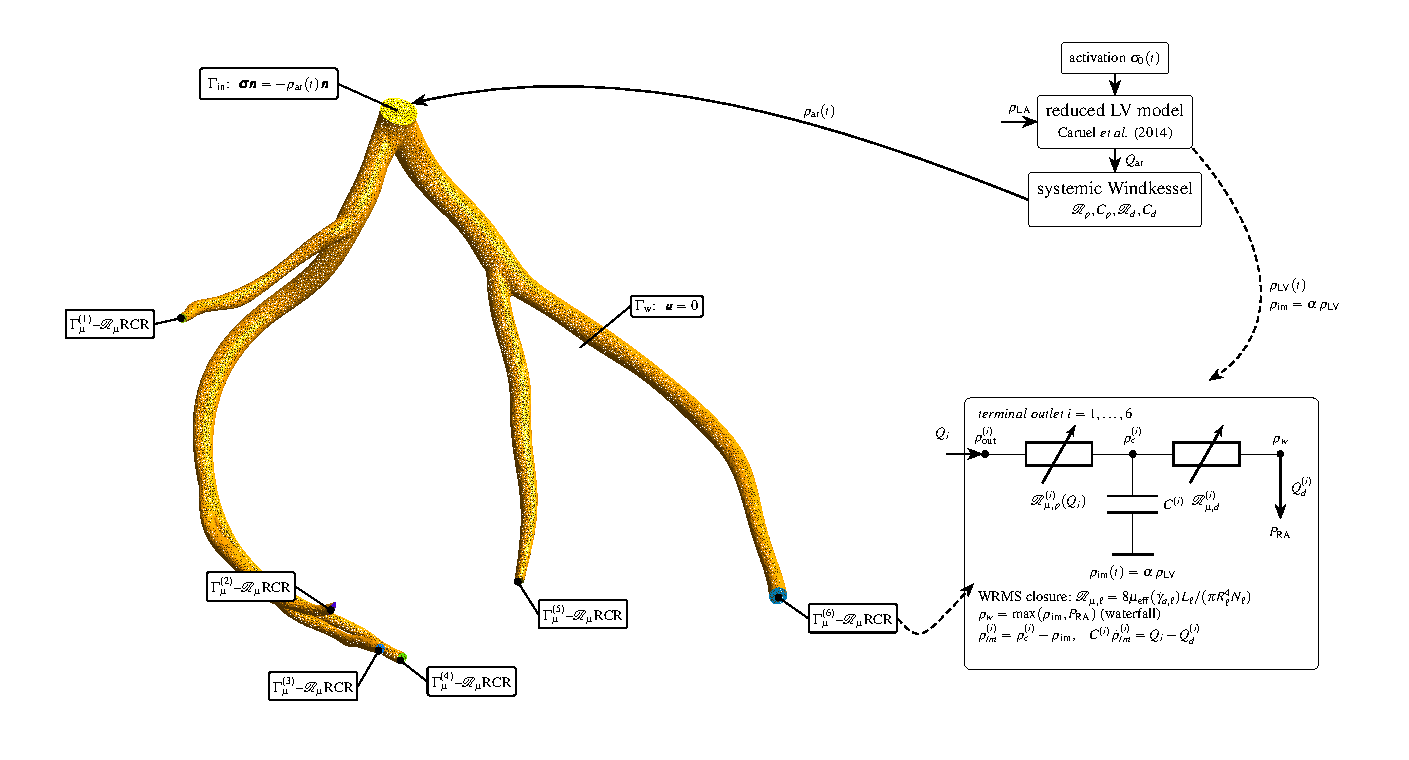
\includegraphics[width=0.98\textwidth]{coronary_setup_rcrmu.pdf}
    \caption{Coupled LV-0D/coronary-3D configuration. The reduced
    left-ventricular model supplies the arterial pressure $p_{\rm ar}(t)$,
    imposed as a normal traction at the coronary inlet
    $\Gamma_{\rm in}$, and the ventricular pressure $p_{\rm LV}(t)$, which
    sets the intramyocardial pressure $p_{\rm im}=\alpha p_{\rm LV}$ acting
    externally on every terminal compartment. No-slip conditions hold on the
    arterial wall $\Gamma_{\rm w}$. Each of the six terminal outlets
    $\Gamma_\mu^{(i)}$ carries the single-state reduced model
    \eqref{eq:coronary-node-balance}--\eqref{eq:coronary-outlet-pressure}
    (inset): a proximal rheology-dependent resistance
    $\mathcal{R}_{\mu,p}^{(i)}$, the transmural pressure state
    $p_{tm}^{(i)}$ on the compliance $C^{(i)}$ referenced to
    $p_{\rm im}$, and a distal rheology-dependent resistance
    $\mathcal{R}_{\mu,d}^{(i)}$ draining through the Starling-type waterfall
    pressure $p_w=\max(p_{\rm im},P_{\rm RA})$ towards the right-atrial
    reservoir $P_{\rm RA}$.}
    \label{fig:coronary-setup}
\end{figure}
% -----------------------------------------------------------------------------
\subsection{Numerical implementation}
\label{sec:numerical-discretisation}
The proximal resistance enters the weak traction operator at each outlet.
During a linear solve,
$\mathcal{R}_{\mu,p}^{(i)}$ is evaluated from the lagged constitutive state and
held fixed. If the normal outlet velocity is represented by its sectional mean,
\begin{equation}
\int_{\Gamma_\mu^{(i)}}
\mathcal{R}_{\mu,p}^{(i)}Q_i
(\boldsymbol{v}\cdot\boldsymbol{n})\,\mathrm{d}\Gamma
\simeq
\mathcal{R}_{\mu,p}^{(i)}A_i
\int_{\Gamma_\mu^{(i)}}
(\boldsymbol{u}\cdot\boldsymbol{n})
(\boldsymbol{v}\cdot\boldsymbol{n})\,\mathrm{d}\Gamma ,
\label{eq:coronary-implicit-resistance}
\end{equation}
where $A_i$ is the outlet area. For
$\mathcal{R}_{\mu,p}^{(i)}>0$, the right-hand side defines a symmetric
positive-semidefinite contribution. The approximation becomes exact for a
spatially uniform normal velocity.
The mesh contains approximately $35\,000$ tetrahedra, $11\,000$ vertices and
$19\,000$ boundary faces and is partitioned over 30 MPI ranks. Taylor--Hood
finite elements \citep{TaylorHood1973} are used,
\begin{equation}
\boldsymbol{u}_h\in[\mathbb{P}_2]^3,
\qquad
p_h\in\mathbb{P}_1,
\end{equation}
with $264\,768$ velocity and $14\,135$ pressure unknowns, giving
$278\,903$ flow degrees of freedom.
The Carreau--Yasuda viscosity is evaluated at the regularised shear rate
\begin{equation}
\dot{\gamma}_{\varepsilon}
=
\left(
\varepsilon_{\gamma}^{2}
+\dot{\gamma}^{2}
\right)^{1/2},
\qquad
\varepsilon_{\gamma}=10^{-3}\,\mathrm{s^{-1}},
\label{eq:regularised-shear-rate}
\end{equation}
where $\dot\gamma$ is defined by \eqref{eq:shear-rate}. The variational
formulation additionally contains the stabilisation terms of the coupled
problem: the Temam divergence correction of the convective term
\citep{Temam2001}, backflow stabilisation at the inlet and at every outlet
\citep{EsmailyMoghadam2011} with unit damping multiplier
$\tfrac12\rho\,(\boldsymbol{u}_{\rm old}\cdot\boldsymbol{n})^{-}$, a weak
normal-impedance term at the inlet with coefficient
$5\times10^{2}\,\mathrm{Pa\,s\,m^{-1}}$, a tangential-penalty term at the
inlet with coefficient $10^{3}$, and a pressure regularisation with
coefficient $10^{-12}$. The Taylor--Hood pair is inf-sup stable; the
pressure regularisation is retained only to fix the hydrostatic pressure mode
for the direct factorisation and is far below the discretisation error.
{\color{red}[Oscar: a mesh-independence assessment for the principal
quantities in \S\ref{sec:results} is still pending and should be added, at
minimum as a comparison against one finer mesh.]}
Time integration is first order and semi-implicit, with time-step size
$\Delta t=10^{-3}\,\mathrm{s}$; when a linear solve fails, the step is
retried with $\Delta t$ halved, up to eight levels, and the nominal step is
recovered afterwards. The linearised saddle-point problem of each step is
solved with a direct factorisation (MUMPS LU through PETSc). The scalar
outlet updates use a Newton iteration with absolute step tolerance
$10^{-9}\,\mathrm{Pa}$ on $p_{tm}^{(i)}$ and at most $50$ iterations; the
rheological closure is evaluated through a log-log tabulation of the WRMS
map with $241$ nodes over $\tau_w\in[10^{-6},10^{4}]\,\mathrm{Pa}$, whose
maximum interpolation error is $0.09\%$. The convective term is linearised
by an Oseen--Picard iteration \citep{ElmanSilvesterWathen2014}. The
advecting velocity, Temam correction \citep{Temam2001}, Carreau--Yasuda
viscosity and the constitutive factors entering the outlet resistances are
taken from the previous time level. One linearised saddle-point problem is
solved per time step.
The coupling is staggered. The LV-0D system is advanced first to obtain
$p_{\rm ar}^{n+1}$ and $p_{\rm LV}^{n+1}$. The three-dimensional problem is
then solved with $p_{\rm ar}^{n+1}$ prescribed at the inlet. The linear
resistive contribution is assembled through
\eqref{eq:coronary-implicit-resistance}, while
$p_{\rm im}+p_{tm}^{(i)}$ is taken from the previous outlet state. The computed
fluxes $Q_i^{n+1}$ are then used to update the six scalar states
$p_{tm}^{(i)}$.
The constitutive coefficients and compartmental pressure are therefore lagged
by one time level, while the linear resistance remains in the
three-dimensional operator. The tangent in \eqref{eq:exact-derivative} is not
used by this semi-implicit scheme. At fixed haematological state, the
Carreau--Yasuda parameter set of the three-dimensional domain is identical
between the $\mathcal{R}_{\mu}$ and constant-outlet calculations.
{\color{red}[Oscar: a temporal-independence check with at least one smaller
$\Delta t$ is still pending and should be reported alongside the mesh
study.]}
% -----------------------------------------------------------------------------
\subsection{Simulation protocol}
\label{sec:simulation-protocol}
The coupled calculations use the healthy, type~2 diabetic and hyperviscous
Carreau--Yasuda parameterisations of \S\ref{sec:pathologies}. Two outlet
closures are evaluated for each state:
\begin{equation}
\begin{aligned}
&\text{$\mathcal{R}_{\mu}$ case:}
&&
\mathcal{R}_{\mu}
=
\mathcal{R}_{\mu}(\Delta p;\boldsymbol\theta),
\\
&\text{constant case:}
&&
\mathcal{R}_{\infty}
=
\frac{8\mu_\infty L}{N\pi R^4}.
\end{aligned}
\label{eq:simulation-cases}
\end{equation}
The state-specific Carreau--Yasuda rheology in the three-dimensional domain is
unchanged between these two calculations. Differences within a state therefore
measure the effect of retaining the shear dependence of the unresolved
resistive compartments. Comparisons between states contain both the bulk
three-dimensional and reduced-outlet rheological changes.
The lumped constants of each outlet follow from an anatomical calibration:
the outlet areas are measured on the mesh, the total resting coronary flow
$Q_{\rm tot}=1.5\times10^{-6}\,\mathrm{m^{3}\,s^{-1}}$ is distributed across
the six outlets by Murray's law
($Q_i\propto r_i^{3}$), the venular fraction $f_v=0.13$ of the resting
pressure budget fixes the split between proximal and distal resistances, and
the total microvascular compliance
$C_{\rm tot}=4\times10^{-10}\,\mathrm{m^{3}\,Pa^{-1}}$ is divided by the
same Murray weights. The reference (Newtonian calibration) viscosity is
$\mu_{\rm ref}=3.5\,\mathrm{mPa\,s}$.
The right-atrial reservoir pressure is fixed at
$P_{\rm RA}=1000\,\mathrm{Pa}$ in all reported calculations. Variation of the
distal rheological operating point is generated by the cardiac-cycle dependence
of $p_{\rm im}$ and the resulting pressure drop across the terminal
compartments.
{\color{red}[Oscar: the value $P_{\rm RA}=1000\,\mathrm{Pa}$
($\approx7.5$~mmHg, upper-normal right-atrial pressure) is stated here and
in the compiled proposal, but the current default in
\texttt{CoupledLV0DCoronary3D.h} is $1800\,\mathrm{Pa}$. Confirm which value
generated the reported results and reconcile the code default before
submission; cite a standard reference for normal right-atrial pressure.]}
%----------------------------------------
% =============================================================================
\section{Results}
\label{sec:results}
Here \emph{resting} refers to the fixed-tone configuration used in the
calculations; vascular tone, vasodilatory reserve and autoregulatory adjustment
of the reduced parameters are not varied.
For each resistive element $\ell\in\{p,d\}$, the representative hydraulic
shear-rate scale is
\begin{equation}
\dot{\gamma}_{a,\ell}(t)
=
\dot{\gamma}_{a,0,\ell}
\frac{|Q_\ell(t)|}{Q_{0,\ell}},
\qquad
\dot{\gamma}_{a,0,\ell}
=
\frac{4\bar v_\ell}{r_\ell},
\label{eq:results-shear-rate}
\end{equation}
where $Q_{0,\ell}$ is the reference flow associated with the corresponding
operating point. The effective hydraulic viscosity satisfies
\begin{equation}
\tau_{w,\ell}
=
\mu_{{\rm eff},\ell}
\dot{\gamma}_{a,\ell}.
\label{eq:results-effective-viscosity}
\end{equation}
The quantity $\dot{\gamma}_{a,\ell}$ is not the constitutive wall shear rate
$\dot{\gamma}_{w,\ell}$; the latter follows from
$\tau_w=\mu(\dot{\gamma}_w)\dot{\gamma}_w$.
Cycle averages are evaluated as
\begin{equation}
\langle f\rangle
=
\frac{1}{t_1-t_0}
\int_{t_0}^{t_1}
f(t)\,\mathrm{d}t.
\label{eq:cycle-average}
\end{equation}
For a cycle-averaged quantity $X$, the change of state $s$ relative to the
healthy state at the same outlet closure is
\begin{equation}
\Delta_X^{(s)}
=
\frac{
\langle X\rangle^{(s)}
-
\langle X\rangle^{({\rm healthy})}
}{
\langle X\rangle^{({\rm healthy})}
}.
\label{eq:state-change}
\end{equation}
At fixed haematological state, the instantaneous coronary-flow difference
between the two outlet closures is
\begin{equation}
E_Q(t)
=
\frac{
|Q_{\rm in}^{\mathcal{R}_{\mu}}(t)|
-
|Q_{\rm in}^{\mu_\infty}(t)|
}{
|Q_{\rm in}^{\mu_\infty}(t)|
}.
\label{eq:closure-flow-error}
\end{equation}
% -----------------------------------------------------------------------------
\subsection{Flow response and reduced wall stress}
\label{sec:results-wall-loading}
For each effective fully developed compartment,
\begin{equation}
\tau_w
=
\frac{R\Delta p}{2L}.
\label{eq:results-wall-stress}
\end{equation}
At fixed $\Delta p$, $R$ and $L$, the reduced wall stress contains no
constitutive parameter. Rheology instead changes the shear rate and discharge
associated with that stress.
In the coupled calculation, healthy and hyperviscous blood produce clearly
separated effective-viscosity histories,
whereas the corresponding reduced wall-stress histories remain much closer.
From healthy to hyperviscous blood, the cycle-averaged wall stress changes by
approximately $-0.4\%$ in the proximal element and $+4.3\%$ in the distal
element, while mean coronary inflow decreases by approximately $15.4\%$.
The non-zero changes in $\tau_w$ arise from changes in the coupled pressure
drops, not from a direct constitutive term in
\eqref{eq:results-wall-stress}. In the resolved three-dimensional arteries,
the wall shear stress also changes indirectly because the outlet closure
modifies the velocity and pressure fields.
\begin{figure}
    \centering
    % Replace by the final Figure 6:
    % \includegraphics[width=\textwidth]{<figure_effective_viscosity_wss>}
    \fbox{
    \rule{0pt}{0.35\textheight}
    \rule{0.92\textwidth}{0pt}
    }
    \caption{Effective hydraulic viscosity $\mu_{\rm eff}$ and reduced wall
    shear stress $\tau_w$ over one cardiac cycle for the proximal and distal
    compartments. Solid lines denote $\mathcal{R}_{\mu}$ and dashed lines the
    state-specific constant resistance based on $\mu_\infty$. Results are shown
    for healthy, type~2 diabetic and hyperviscous blood. The shaded interval
    denotes systole.
    {\color{red}[Oscar: replace $\mu_{\rm ap}$ by $\mu_{\rm eff}$ in the final
    artwork and verify the reported cycle-averaged percentages from the final
    data.]}}
    \label{fig:cycle-viscosity-wallstress}
\end{figure}
% -----------------------------------------------------------------------------
\subsection{Operating range of the coronary compartments}
\label{sec:results-operating-point}
Using \eqref{eq:gamma-velocity}, the reference apparent shear-rate scales are
approximately $800\,\mathrm{s}^{-1}$ for the proximal compartment
($r=25\,\mu\mathrm{m}$, $\bar v=5\,\mathrm{mm\,s^{-1}}$) and
$400\,\mathrm{s}^{-1}$ for the distal compartment
($r=30\,\mu\mathrm{m}$, $\bar v=3\,\mathrm{mm\,s^{-1}}$).
The corresponding reference wall stresses are approximately $2.8$ and
$1.4\,\mathrm{Pa}$.
Across the three haematological states, the cycle-averaged proximal
$\dot{\gamma}_a$ lies between approximately $343$ and
$406\,\mathrm{s}^{-1}$, and the distal value between approximately
$186$ and $216\,\mathrm{s}^{-1}$. Both compartments therefore spend most of
the cycle in the high-shear portion of the plateau-preserving constitutive
responses.
The location of these operating points explains why a resistance based on the
high-shear viscosity remains close to $\mathcal{R}_{\mu}$ for the
cycle-averaged flow under the fixed-tone conditions considered here.
{\color{red}[Oscar: verify the sources and final values of the representative
radii, velocities and wall-stress estimates. These quantities support the
a priori operating-point argument and should be linked directly to coronary
microvascular data (intravital microscopy reports arteriolar calibres and
red-cell velocities in these ranges; add the specific references). The values
quoted here match the implementation
($r_a=25\,\mu$m, $\bar v_a=5$\,mm\,s$^{-1}$, $r_v=30\,\mu$m,
$\bar v_v=3$\,mm\,s$^{-1}$). Do not restore the previous transit-time
estimate unless its discrepancy with reported coronary transit times has been
resolved.]}
% -----------------------------------------------------------------------------
\subsection{Cardiac-cycle excursion towards low shear}
\label{sec:results-cycle-excursion}
Systolic intramyocardial compression reduces the pressure drop and flow through
the terminal compartments and moves their operating points towards lower
$\dot{\gamma}_a$.
We quantify departure from the high-shear plateau by defining
$\dot{\gamma}_{a,\rm tr}$ from
\begin{equation}
\mu_{\rm eff}
\left(
\dot{\gamma}_{a,\rm tr}
\right)
=
(1+\varepsilon)\mu_\infty.
\label{eq:transition-shear-rate}
\end{equation}
Hence,
$\dot{\gamma}_a<\dot{\gamma}_{a,\rm tr}$
identifies conditions for which the effective hydraulic viscosity exceeds
$\mu_\infty$ by more than the prescribed fraction $\varepsilon$. This
criterion refers only to departure from the high-shear hydraulic response and
does not define an erythrocyte-aggregation threshold.
For $\varepsilon=0.2$,
$\dot{\gamma}_{a,\rm tr}$ is approximately $47$, $25$ and
$108\,\mathrm{s}^{-1}$ for the healthy, type~2 diabetic and hyperviscous
parameterisations. For $\varepsilon=0.1$, the corresponding values are
approximately $110$, $56$ and $257\,\mathrm{s}^{-1}$. The hyperviscous
parameterisation therefore departs from its high-shear plateau at larger
$\dot{\gamma}_a$ than the healthy and diabetic parameterisations.
During systolic compression, the proximal flow approaches zero and
$\mu_{\rm eff}$ moves rapidly towards its low-shear value. Because the
transported flow is small over this interval, the large instantaneous
viscosity change contributes little to cycle-integrated coronary transport.
The distal compartment continues to conduct and reaches
$\dot{\gamma}_a\approx28$--$33\,\mathrm{s}^{-1}$, placing it within the
low-shear transition range while maintaining finite outflow.
\begin{figure}
    \centering
    % Replace by the final Figure 7:
    % \includegraphics[width=\textwidth]{<figure_coronary_inflow_distal_shear>}
    \fbox{
    \rule{0pt}{0.29\textheight}
    \rule{0.92\textwidth}{0pt}
    }
    \caption{Coronary inflow and distal representative hydraulic shear-rate
    scale over one cardiac cycle. Solid lines denote $\mathcal{R}_{\mu}$ and
    dashed lines the corresponding state-specific constant resistance based on
    $\mu_\infty$. The horizontal line marks
    $\dot\gamma_{a,0}=400\,\mathrm{s}^{-1}$. The low-shear region is defined
    from the healthy-state criterion \eqref{eq:transition-shear-rate} with
    $\varepsilon=0.2$ and is included only as a constitutive reference. The
    shaded time interval denotes systole.
    {\color{red}[Oscar: replace the current label ``Aggregation Regime'' by
    ``Low-shear transition region'' or equivalent. The generalised-Newtonian
    model does not define a kinetic aggregation threshold.]}}
    \label{fig:cycle-flow-shear}
\end{figure}
The low-flow proximal excursion should not be interpreted as a prediction of
the degree of erythrocyte aggregation during systole. The
generalised-Newtonian constitutive law responds instantaneously to
$\dot{\gamma}$ and contains no aggregation or disaggregation time scale.
A transient low-shear interval shorter than the relevant structural relaxation
time cannot be resolved by this constitutive description.
{\color{red}[Oscar: add a blood-rheology reference supporting the finite
time scale of aggregation/disaggregation. Do not introduce a numerical
relaxation time unless it is supported directly by experimental data.]}
% -----------------------------------------------------------------------------
\subsection{Viscosity level and shear-dependent resistance}
\label{sec:results-state-vs-sheardependence}
With $\mathcal{R}_{\mu}$ at the terminal compartments, mean coronary inflow is
approximately $8.1\%$ lower for type~2 diabetic blood and $15.4\%$ lower for
the hyperviscous state than for healthy blood. When all three states instead
use their corresponding constant outlet resistances based on $\mu_\infty$, the
hyperviscous case still gives an approximately $11.9\%$ reduction relative to
healthy blood.
Most of the healthy-to-hyperviscous inflow difference therefore remains when
the shear dependence of the terminal resistance is removed. For these
parameterisations and this operating range, the dominant contribution arises
from the difference in viscosity level, while the additional reduction obtained
with $\mathcal{R}_{\mu}$ is associated with departure from the high-shear
plateau during the cardiac cycle.
A state-to-state flow difference cannot by itself quantify the
shear-dependent contribution. That contribution is obtained from the
fixed-state comparison between $\mathcal{R}_{\mu}$ and the corresponding
constant outlet resistance.
\begin{figure}
    \centering
    % Replace by the final Figure 8:
    % \includegraphics[width=\textwidth]{<figure_cycle_averaged_changes>}
    \fbox{
    \rule{0pt}{0.30\textheight}
    \rule{0.92\textwidth}{0pt}
    }
    \caption{Changes in cycle-averaged quantities relative to healthy blood for
    the type~2 diabetic and hyperviscous states. Quantities shown are coronary
    inflow, proximal and distal effective hydraulic viscosity
    $\mu_{\rm eff}$, and proximal and distal reduced wall shear stress
    $\tau_w$. Solid bars denote $\mathcal{R}_{\mu}$ and hatched bars the
    state-specific constant resistance based on $\mu_\infty$.
    {\color{red}[Oscar: use $\mu_{\rm eff}$ rather than $\mu_{\rm ap}$ in the
    final artwork and verify all percentages from the final cycle-averaged
    data.]}}
    \label{fig:state-cycle-averages}
\end{figure}
% -----------------------------------------------------------------------------
\subsection{Error of the high-shear constant resistance}
\label{sec:results-constant-resistance}
At fixed haematological state, replacing $\mathcal{R}_{\mu}$ by the
resistance based on $\mu_\infty$ changes the cycle-averaged coronary inflow by
approximately $3.4\%$ for healthy blood, $2.0\%$ for type~2 diabetic blood and
$7.4\%$ for the hyperviscous state. The same approximation underestimates the
cycle-averaged effective hydraulic viscosity by approximately $8.6\%$,
$5.2\%$ and $24.6\%$, respectively.
The hyperviscous parameterisation gives the largest discrepancy because its
hydraulic response remains shear dependent over a larger fraction of the
coronary operating range. The diabetic parameterisation, although more viscous
than the healthy one, lies closer to its high-shear plateau over the same
range and produces the smallest closure correction.
Instantaneous discrepancies are larger during systolic low-flow intervals.
The ratio
$\mu_{\rm eff}^{\mathcal{R}_{\mu}}/\mu_\infty$
can exceed an order of magnitude near proximal flow closure. This occurs when
the transported flow is close to zero and is therefore not representative of
the effect on cycle-averaged coronary transport.
\begin{figure}
    \centering
    % Replace by the final Figure 9:
    % \includegraphics[width=\textwidth]{<figure_constant_resistance_error>}
    \fbox{
    \rule{0pt}{0.29\textheight}
    \rule{0.92\textwidth}{0pt}
    }
    \caption{Departure of the state-specific constant outlet resistance based
    on $\mu_\infty$ from $\mathcal{R}_{\mu}$ over one cardiac cycle. Left:
    coronary-inflow difference $E_Q$ defined by
    \eqref{eq:closure-flow-error}. Right:
    $\mu_{\rm eff}^{\mathcal{R}_{\mu}}/\mu_\infty$.
    Results are shown for healthy, type~2 diabetic and hyperviscous blood; the
    shaded interval denotes systole.
    {\color{red}[Oscar: update the right-hand ordinate to
    $\mu_{\rm eff}^{\mathcal{R}_{\mu}}/\mu_\infty$ and verify the sign
    convention of $E_Q$ against \eqref{eq:closure-flow-error}.]}}
    \label{fig:constant-resistance-error}
\end{figure}
% -----------------------------------------------------------------------------
\subsection{Range of the numerical experiment}
\label{sec:results-consistency}
The transmural pressure remains positive throughout the cardiac cycle for all
three haematological states. Its minimum values are approximately
$1175$, $1205$ and $1256\,\mathrm{Pa}$ for healthy, type~2 diabetic and
hyperviscous blood, respectively. The single-state terminal model therefore
remains in the positive-transmural-pressure range sampled by the present
calculations.
The six outlets carry different fractions of the total coronary flow but
remain within the same broad rheological operating range.
The operating point is varied only through phasic intramyocardial loading; no
independent variation of right-atrial pressure or vascular tone is included.
State-to-state comparisons change both the three-dimensional constitutive law
and the reduced terminal rheology, whereas fixed-state closure comparisons
change only the terminal resistance. The generalised-Newtonian law contains no
structural relaxation time and does not resolve aggregation kinetics during
short low-shear excursions.
{\color{red}[Oscar: verify the minimum transmural pressures from the final
periodic solutions and the outlet flow-share range if it is retained. Do not
restore the previous analytical bound on $p_{tm}$ unless it is derived
explicitly from the final Starling-resistor model.]}
%---------------------------------------
\section{Conclusions}
\label{sec:conclusions}
A generalised-Newtonian constitutive law can be transferred to the
pressure--flow relation of an unresolved vascular compartment through the
WRMS formulation. The hydraulic resistance $\mathcal{R}_{\mu}$ then depends
on the operating pressure drop through the constitutive stress--shear-rate
relation and reduces to the Hagen--Poiseuille resistance in the Newtonian
limit. The construction applies to the power-law, Cross, Carreau--Yasuda and
Quemada models considered here.
For prescribed effective radius, path length and pressure drop, the axial
momentum balance fixes the wall shear stress independently of the constitutive
law. These quantities set the stress scale sampled by the unresolved
compartment and provide an a priori estimate of its rheological operating
range. A constant resistance is appropriate when that range remains close to
a viscosity plateau; it ceases to represent the pressure--flow response as the
operating point traverses a shear-dependent part of the constitutive curve.
Haematocrit and haematological state enter the reduced model through the
constitutive parameters defining $\mathcal{R}_{\mu}$, without an additional
rheological term in the Windkessel equations. The same nonlinear resistive
element can be used in lumped models or as a distal pressure--flow condition
for a higher-dimensional solver. Its analytical pressure--flow derivative
provides the tangent required by Newton or monolithic coupling strategies.
The closure inherits the assumptions of the bulk generalised-Newtonian
description. It contains no constitutive memory and does not resolve
aggregation or disaggregation kinetics. Haematocrit is represented by an
effective cross-sectional concentration, so radial cell migration and the
F\aa hr\ae us and F\aa hr\ae us--Lindqvist effects are not resolved
explicitly. The vascular bed is represented through effective geometrical
parameters rather than distributions of vessel calibre and path length.
These assumptions delimit the spatial and temporal scales for which
$\mathcal{R}_{\mu}$ represents the unresolved pressure--flow response.
%%%%%%%%%%%%%%%%%%%%%%%%%%%%%%%%%%%%%%%%%%%%%%%%%%%%%%%%%%%%%%%%%%%%%%%%%%%%%%%
% APPENDICES
%%%%%%%%%%%%%%%%%%%%%%%%%%%%%%%%%%%%%%%%%%%%%%%%%%%%%%%%%%%%%%%%%%%%%%%%%%%%%%%
\appendix
% =============================================================================
\section{Analytical evaluation of the rheological integral for the Cross and
Carreau--Yasuda models}
\label{appA}
\subsection{Cross model}
For the Cross model, the rheological integral in \eqref{Int:Cross} has
integrand
\[
\dot\gamma^{3}\mu(\dot\gamma)^{2}
\frac{\mathrm{d}\tau}{\mathrm{d}\dot\gamma}.
\]
With $\delta=\mu_0-\mu_\infty$, direct expansion gives
\begin{align}
I_1
&=
\int_0^{\dot{\gamma}_w}
\mu_{\infty}^3\dot{\gamma}^3
\,\mathrm{d}\dot{\gamma}
=
\frac{\mu_{\infty}^3\dot{\gamma}_w^4}{4},
\\[6pt]
I_2
&=
3\mu_{\infty}^2\delta
\int_0^{\dot{\gamma}_w}
\frac{\dot{\gamma}^3}
{1+(\lambda\dot{\gamma})^n}
\,\mathrm{d}\dot{\gamma},
\\[6pt]
I_3
&=
3\mu_{\infty}\delta^2
\int_0^{\dot{\gamma}_w}
\frac{\dot{\gamma}^3}
{\left(1+(\lambda\dot{\gamma})^n\right)^2}
\,\mathrm{d}\dot{\gamma},
\\[6pt]
I_4
&=
-\mu_{\infty}^2n\delta
\int_0^{\dot{\gamma}_w}
\frac{(\lambda\dot{\gamma})^n\dot{\gamma}^3}
{\left(1+(\lambda\dot{\gamma})^n\right)^2}
\,\mathrm{d}\dot{\gamma},
\\[6pt]
I_5
&=
\delta^3
\int_0^{\dot{\gamma}_w}
\frac{\dot{\gamma}^3}
{\left(1+(\lambda\dot{\gamma})^n\right)^3}
\,\mathrm{d}\dot{\gamma},
\\[6pt]
I_6
&=
-2\mu_{\infty}\delta^2n
\int_0^{\dot{\gamma}_w}
\frac{(\lambda\dot{\gamma})^n\dot{\gamma}^3}
{\left(1+(\lambda\dot{\gamma})^n\right)^3}
\,\mathrm{d}\dot{\gamma},
\\[6pt]
I_7
&=
-n\delta^3
\int_0^{\dot{\gamma}_w}
\frac{(\lambda\dot{\gamma})^n\dot{\gamma}^3}
{\left(1+(\lambda\dot{\gamma})^n\right)^4}
\,\mathrm{d}\dot{\gamma}.
\end{align}
Terms without the additional factor $(\lambda\dot\gamma)^n$ belong to
\begin{equation}
J_k^{\mathrm{Cr}}
=
\int_0^{\dot{\gamma}_w}
\frac{\dot{\gamma}^3}
{\left(1+(\lambda\dot{\gamma})^n\right)^k}
\,\mathrm{d}\dot{\gamma},
\label{eq:app-J-Cross}
\end{equation}
with
\begin{equation}
J_k^{\mathrm{Cr}}
=
\frac{\dot{\gamma}_w^4}{4}
{}_2F_1\!\left(
k,\frac{4}{n};
1+\frac{4}{n};
-(\lambda\dot{\gamma}_w)^n
\right).
\label{eq:app-J-Cross-hyper}
\end{equation}
For terms containing $(\lambda\dot\gamma)^n$, define
\begin{equation}
K_k^{\mathrm{Cr}}
=
\int_0^{\dot{\gamma}_w}
\frac{\dot{\gamma}^3(\lambda\dot{\gamma})^n}
{\left(1+(\lambda\dot{\gamma})^n\right)^k}
\,\mathrm{d}\dot{\gamma}.
\label{eq:app-K-Cross}
\end{equation}
Using
\begin{equation}
\frac{(\lambda\dot{\gamma})^n}
{\left(1+(\lambda\dot{\gamma})^n\right)^k}
=
\frac{1}
{\left(1+(\lambda\dot{\gamma})^n\right)^{k-1}}
-
\frac{1}
{\left(1+(\lambda\dot{\gamma})^n\right)^k},
\end{equation}
gives
\begin{equation}
K_k^{\mathrm{Cr}}
=
J_{k-1}^{\mathrm{Cr}}
-
J_k^{\mathrm{Cr}}.
\label{eq:app-KJ-Cross}
\end{equation}
Collecting equal powers yields
\begin{align}
I_{\mathrm{Cr}}
&=
\mu_{\infty}^3J_0^{\mathrm{Cr}}
+\mu_{\infty}^2\delta(3-n)J_1^{\mathrm{Cr}}
\nonumber\\
&\quad
+\left[
\mu_{\infty}\delta^2(3-2n)
+\mu_{\infty}^2n\delta
\right]J_2^{\mathrm{Cr}}
\nonumber\\
&\quad
+\left[
\delta^3(1-n)
+2\mu_{\infty}\delta^2n
\right]J_3^{\mathrm{Cr}}
+n\delta^3J_4^{\mathrm{Cr}},
\label{eq:app-I-Cross}
\end{align}
which is the expression used in \eqref{eq:I_Cross_expanded}.
Expression \eqref{eq:app-I-Cross} was verified against direct adaptive
quadrature of \eqref{eq:I_gamma_form} for the three Cross parameter sets of
table~\ref{tab:rheology} at wall stresses spanning the low-shear, transition
and high-shear ranges ($\tau_w=10^{-4}$--$10^{2}\,\mathrm{Pa}$); the maximum
relative discrepancy is $3\times10^{-13}$, and the limit
$\mu_0\rightarrow\mu_\infty$ reproduces the Newtonian integral
$\tau_w^4/(4\mu)$ to machine precision.
% -----------------------------------------------------------------------------
\subsection{Carreau--Yasuda model}
For the Carreau--Yasuda model,
\begin{equation}
I_{\mathrm{CY}}
=
\int_0^{\dot\gamma_w}
\dot\gamma^3
\mu(\dot\gamma)^2
\frac{\mathrm{d}\tau}{\mathrm{d}\dot\gamma}
\,\mathrm{d}\dot\gamma .
\label{eq:app-I-CY-definition}
\end{equation}
Define
\begin{equation}
\chi
=
1+(\lambda\dot\gamma)^a,
\qquad
b
=
\frac{n-1}{a},
\label{eq:app-chi-CY}
\end{equation}
so that
\begin{equation}
\mu(\dot\gamma)
=
\mu_\infty+\delta\chi^b,
\qquad
\delta=\mu_0-\mu_\infty .
\label{eq:app-mu-CY}
\end{equation}
Differentiation of
$\tau=\mu(\dot\gamma)\dot\gamma$ gives
\begin{equation}
\frac{\mathrm{d}\tau}{\mathrm{d}\dot\gamma}
=
\mu_\infty
+\delta\chi^b
+\delta(n-1)
(\lambda\dot\gamma)^a\chi^{b-1}.
\label{eq:dtau_CY}
\end{equation}
Since $(\lambda\dot\gamma)^a=\chi-1$,
\eqref{eq:dtau_CY} is equivalent to
\eqref{eq:dtau_dgamma_CY}.
Substitution into \eqref{eq:app-I-CY-definition} gives
\begin{align}
I_{\mathrm{CY}}
&=
\int_0^{\dot{\gamma}_w}
\dot{\gamma}^3
\left(\mu_{\infty}+\delta\chi^b\right)^2
\nonumber\\
&\qquad\times
\left[
\mu_{\infty}
+\delta\chi^b
+\delta(n-1)
(\lambda\dot{\gamma})^a\chi^{b-1}
\right]
\,\mathrm{d}\dot{\gamma}.
\label{eq:app-I-CY-start}
\end{align}
Expansion gives
\begin{align}
I_{\mathrm{CY}}
&=
\int_0^{\dot\gamma_w}
\dot\gamma^3
\Big[
\mu_\infty^3
+3\mu_\infty^2\delta\chi^b
+\mu_\infty^2\delta(n-1)
(\lambda\dot\gamma)^a\chi^{b-1}
\nonumber\\
&\qquad
+3\mu_\infty\delta^2\chi^{2b}
+2\mu_\infty\delta^2(n-1)
(\lambda\dot\gamma)^a\chi^{2b-1}
\nonumber\\
&\qquad
+\delta^3\chi^{3b}
+\delta^3(n-1)
(\lambda\dot\gamma)^a\chi^{3b-1}
\Big]
\,\mathrm{d}\dot\gamma .
\label{eq:app-I-CY-expanded}
\end{align}
Using
\begin{equation}
(\lambda\dot\gamma)^a=\chi-1
\label{eq:app-CY-identity}
\end{equation}
reduces all terms to
\begin{equation}
J_k^{\mathrm{CY}}
=
\int_0^{\dot{\gamma}_w}
\dot{\gamma}^3
\left(1+(\lambda\dot{\gamma})^a\right)^k
\,\mathrm{d}\dot{\gamma},
\label{eq:app-J-CY-definition}
\end{equation}
with
\begin{equation}
J_k^{\mathrm{CY}}
=
\frac{\dot{\gamma}_w^4}{4}
{}_2F_1\!\left(
-k,\frac{4}{a};
1+\frac{4}{a};
-(\lambda\dot{\gamma}_w)^a
\right).
\label{eq:app-J-CY}
\end{equation}
Hence,
\begin{align}
I_{\mathrm{CY}}
&=
\mu_\infty^3J_0^{\mathrm{CY}}
+\mu_\infty^2\delta(n+2)J_b^{\mathrm{CY}}
-\mu_\infty^2\delta(n-1)J_{b-1}^{\mathrm{CY}}
\nonumber\\
&\quad
+\mu_\infty\delta^2(2n+1)J_{2b}^{\mathrm{CY}}
-2\mu_\infty\delta^2(n-1)J_{2b-1}^{\mathrm{CY}}
\nonumber\\
&\quad
+\delta^3nJ_{3b}^{\mathrm{CY}}
-\delta^3(n-1)J_{3b-1}^{\mathrm{CY}},
\qquad
b=\frac{n-1}{a},
\label{eq:app-I-CY-final}
\end{align}
which is equivalent to \eqref{eq:I_CY_final}.
Expression \eqref{eq:app-I-CY-final} was verified independently against
direct adaptive quadrature of \eqref{eq:I_gamma_form} for the three
Carreau--Yasuda parameter sets of table~\ref{tab:rheology}, including the
contributions involving $J_{b-1}^{\mathrm{CY}}$, $J_{2b-1}^{\mathrm{CY}}$
and $J_{3b-1}^{\mathrm{CY}}$, over the same low-shear, transition,
high-shear and Newtonian-limit checks used for the Cross model; the maximum
relative discrepancy is $2\times10^{-12}$.
% =============================================================================
\section{Auxiliary coefficients for the analytical Quemada resistance}
\label{appB}
The analytical Quemada resistance of \S\ref{sec:Rmu} is expressed through
$F(\alpha_{\mathrm Q},q_{\mathrm Q})$ in \eqref{eq:F_alpha_q}. The stress
scale $\tau_0$, high-shear viscosity $\mu_\infty$, transformed shear-rate
parameter $\Lambda_{\mathrm Q}$ and dimensionless variables
$\alpha_{\mathrm Q}$ and $q_{\mathrm Q}$ are defined in
\eqref{eq:tau0_quemada}--\eqref{eq:alpha_q}.
The polynomial coefficients entering \eqref{eq:F_alpha_q} are
\begin{align}
P_1
&=
-\tfrac{1}{7}(q_{\mathrm Q}+8),
\\
P_2
&=
-\tfrac{1}{42}
(13q_{\mathrm Q}^2-8q_{\mathrm Q}-7),
\\
P_3
&=
-\tfrac{1}{210}
(143q_{\mathrm Q}^3-88q_{\mathrm Q}^2-113q_{\mathrm Q}+48),
\\
P_4
&=
-\tfrac{1}{840}
(1287q_{\mathrm Q}^4-792q_{\mathrm Q}^3
-1342q_{\mathrm Q}^2+632q_{\mathrm Q}+175),
\\
P_5
&=
-\tfrac{1}{840}
(3003q_{\mathrm Q}^5-1848q_{\mathrm Q}^4
-3894q_{\mathrm Q}^3+1944q_{\mathrm Q}^2
+1011q_{\mathrm Q}-256),
\\
P_6
&=
-\tfrac{1}{1680}
\bigl(
15015q_{\mathrm Q}^6-9240q_{\mathrm Q}^5
-23331q_{\mathrm Q}^4+12096q_{\mathrm Q}^3
+9081q_{\mathrm Q}^2-3179q_{\mathrm Q}-525
\bigr),
\\
P_7
&=
-\tfrac{1}{1680}
\bigl(
45045q_{\mathrm Q}^7-27720q_{\mathrm Q}^6
-82005q_{\mathrm Q}^5+43680q_{\mathrm Q}^4
+42819q_{\mathrm Q}^3
\nonumber\\
&\hspace{2.9cm}
-17304q_{\mathrm Q}^2-5619q_{\mathrm Q}+1024
\bigr),
\\
P_8
&=
-\tfrac{1}{16}
(1-q_{\mathrm Q})^2(1+q_{\mathrm Q})
\left(
429q_{\mathrm Q}^5
+165q_{\mathrm Q}^4
-330q_{\mathrm Q}^3
-90q_{\mathrm Q}^2
+45q_{\mathrm Q}+5
\right).
\end{align}
Together with
\eqref{eq:tau0_quemada}--\eqref{eq:alpha_q}, these coefficients determine
$F(\alpha_{\mathrm Q},q_{\mathrm Q})$ and therefore
$\mathcal{R}_{\mu}^{\mathrm Q}$.
As transcribed above, the coefficients $P_1$--$P_8$ together with
\eqref{eq:tau0_quemada}--\eqref{eq:alpha_q} were checked numerically:
$F(\alpha_{\mathrm Q},q_{\mathrm Q})$ agrees with direct quadrature of
\eqref{eq:I_gamma_form} for the Quemada law to better than
$2\times10^{-4}$ in relative terms for all three haematological states, over
wall stresses spanning the operating range of \S\ref{sec:results}.
{\color{red}[Oscar: the numerical check above validates the internal
consistency of the transcription; a final visual comparison of
$P_1$--$P_8$ against the original \citet{Popel1993} derivation is still
recommended before submission.]}
\bibliographystyle{jfm}
\bibliography{jfm}
% Bibliography is generated from jfm.bib.
\end{document}
